%%%%%%%%%%%%%%%%%%%%%%%%%%%%%%%%%%%%%%%%%
% The Legrand Orange Book
% LaTeX Template
% Version 2.0 (9/2/15)
%
% This template has been downloaded from:
% http://www.LaTeXTemplates.com
%
% Mathias Legrand (legrand.mathias@gmail.com) with modifications by:
% Vel (vel@latextemplates.com)
%
% License:
% CC BY-NC-SA 3.0 (http://creativecommons.org/licenses/by-nc-sa/3.0/)
%
% Compiling this template:
% This template uses biber for its bibliography and makeindex for its index.
% When you first open the template, compile it from the command line with the 
% commands below to make sure your LaTeX distribution is configured correctly:
%
% 1) pdflatex main
% 2) makeindex main.idx -s StyleInd.ist
% 3) biber main
% 4) pdflatex main x 2
%
% After this, when you wish to update the bibliography/index use the appropriate
% command above and make sure to compile with pdflatex several times 
% afterwards to propagate your changes to the document.
%
% This template also uses a number of packages which may need to be
% updated to the newest versions for the template to compile. It is strongly
% recommended you update your LaTeX distribution if you have any
% compilation errors.
%
% Important note:
% Chapter heading images should have a 2:1 width:height ratio,
% e.g. 920px width and 460px height.
%
%%%%%%%%%%%%%%%%%%%%%%%%%%%%%%%%%%%%%%%%%

%----------------------------------------------------------------------------------------
%	PACKAGES AND OTHER DOCUMENT CONFIGURATIONS
%----------------------------------------------------------------------------------------

\documentclass[11pt,fleqn]{book} % Default font size and left-justified equations

%----------------------------------------------------------------------------------------

%%%%%%%%%%%%%%%%%%%%%%%%%%%%%%%%%%%%%%%%%
% The Legrand Orange Book
% Structural Definitions File
% Version 2.0 (9/2/15)
%
% Original author:
% Mathias Legrand (legrand.mathias@gmail.com) with modifications by:
% Vel (vel@latextemplates.com)
% 
% This file has been downloaded from:
% http://www.LaTeXTemplates.com
%
% License:
% CC BY-NC-SA 3.0 (http://creativecommons.org/licenses/by-nc-sa/3.0/)
%
%%%%%%%%%%%%%%%%%%%%%%%%%%%%%%%%%%%%%%%%%

%----------------------------------------------------------------------------------------
%	VARIOUS REQUIRED PACKAGES AND CONFIGURATIONS
%----------------------------------------------------------------------------------------

\usepackage[top=3cm,bottom=3cm,left=3cm,right=3cm,headsep=10pt,a4paper]{geometry} % Page margins

\usepackage[table,xcdraw]{xcolor} % Required for specifying colors by name
\definecolor{ocre}{RGB}{243,102,25} % Define the orange color used for highlighting throughout the book
\definecolor{rightexample}{RGB}{31,181,0}
\definecolor{wrongexample}{RGB}{238,41,18}

% Used for longtables
\usepackage{tabularx}
\usepackage{longtable}
\usepackage{ltxtable}

\usepackage{graphicx} % Required for including pictures
\graphicspath{{Pictures/}} % Specifies the directory where pictures are stored

\usepackage{placeins} % Required for floatbarrier

\usepackage{lipsum} % Inserts dummy text

\usepackage{tikz} % Required for drawing custom shapes

\usepackage[english]{babel} % English language/hyphenation

\usepackage{enumitem} % Customize lists
\setlist{nolistsep} % Reduce spacing between bullet points and numbered lists

\usepackage{booktabs} % Required for nicer horizontal rules in tables

\usepackage{todonotes} % Used in order to make todos

\usepackage{xspace} % Used to make space in commands

% Used for making multiple figures within one figure
\usepackage{wrapfig}
\usepackage{subcaption}

\usepackage{array}

%----------------------------------------------------------------------------------------
%	FONTS
%----------------------------------------------------------------------------------------

\usepackage{avant} % Use the Avantgarde font for headings
%\usepackage{times} % Use the Times font for headings
\usepackage{mathptmx} % Use the Adobe Times Roman as the default text font together with math symbols from the Sym­bol, Chancery and Com­puter Modern fonts

\usepackage{microtype} % Slightly tweak font spacing for aesthetics
\usepackage[utf8]{inputenc} % Required for including letters with accents
\usepackage[T1]{fontenc} % Use 8-bit encoding that has 256 glyphs

%----------------------------------------------------------------------------------------
%	BIBLIOGRAPHY AND INDEX
%----------------------------------------------------------------------------------------

\usepackage[style=alphabetic,citestyle=numeric,sorting=nyt,sortcites=true,autopunct=true,babel=hyphen,hyperref=true,abbreviate=false,backref=true,backend=biber]{biblatex}
\addbibresource{bibliography.bib} % BibTeX bibliography file
\defbibheading{bibempty}{}

\usepackage{calc} % For simpler calculation - used for spacing the index letter headings correctly
\usepackage{makeidx} % Required to make an index
\makeindex % Tells LaTeX to create the files required for indexing

%----------------------------------------------------------------------------------------
%	MAIN TABLE OF CONTENTS
%----------------------------------------------------------------------------------------

\usepackage{titletoc} % Required for manipulating the table of contents

\contentsmargin{0cm} % Removes the default margin

% Part text styling
\titlecontents{part}[0cm]
{\addvspace{20pt}\centering\large\bfseries}
{}
{}
{}

% Chapter text styling
\titlecontents{chapter}[1.25cm] % Indentation
{\addvspace{12pt}\large\sffamily\bfseries} % Spacing and font options for chapters
{\color{ocre!60}\contentslabel[\Large\thecontentslabel]{1.25cm}\color{ocre}} % Chapter number
{\color{ocre}}  
{\color{ocre!60}\normalsize\;\titlerule*[.5pc]{.}\;\thecontentspage} % Page number

% Section text styling
\titlecontents{section}[1.25cm] % Indentation
{\addvspace{3pt}\sffamily\bfseries} % Spacing and font options for sections
{\contentslabel[\thecontentslabel]{1.25cm}} % Section number
{}
{\hfill\color{black}\thecontentspage} % Page number
[]

% Subsection text styling
\titlecontents{subsection}[1.25cm] % Indentation
{\addvspace{1pt}\sffamily\small} % Spacing and font options for subsections
{\contentslabel[\thecontentslabel]{1.25cm}} % Subsection number
{}
{\ \titlerule*[.5pc]{.}\;\thecontentspage} % Page number
[]

% List of figures
\titlecontents{figure}[0em]
{\addvspace{-5pt}\sffamily}
{\thecontentslabel\hspace*{1em}}
{}
{\ \titlerule*[.5pc]{.}\;\thecontentspage}
[]

% List of tables
\titlecontents{table}[0em]
{\addvspace{-5pt}\sffamily}
{\thecontentslabel\hspace*{1em}}
{}
{\ \titlerule*[.5pc]{.}\;\thecontentspage}
[]

%----------------------------------------------------------------------------------------
%	MINI TABLE OF CONTENTS IN PART HEADS
%----------------------------------------------------------------------------------------

% Chapter text styling
\titlecontents{lchapter}[0em] % Indenting
{\addvspace{15pt}\large\sffamily\bfseries} % Spacing and font options for chapters
{\color{ocre}\contentslabel[\Large\thecontentslabel]{1.25cm}\color{ocre}} % Chapter number
{}  
{\color{ocre}\normalsize\sffamily\bfseries\;\titlerule*[.5pc]{.}\;\thecontentspage} % Page number

% Section text styling
\titlecontents{lsection}[0em] % Indenting
{\sffamily\small} % Spacing and font options for sections
{\contentslabel[\thecontentslabel]{1.25cm}} % Section number
{}
{}

% Subsection text styling
\titlecontents{lsubsection}[.5em] % Indentation
{\normalfont\footnotesize\sffamily} % Font settings
{}
{}
{}

%----------------------------------------------------------------------------------------
%	PAGE HEADERS
%----------------------------------------------------------------------------------------

\usepackage{fancyhdr} % Required for header and footer configuration

\pagestyle{fancy}
\renewcommand{\chaptermark}[1]{\markboth{\sffamily\normalsize\bfseries\chaptername\ \thechapter.\ #1}{}} % Chapter text font settings
\renewcommand{\sectionmark}[1]{\markright{\sffamily\normalsize\thesection\hspace{5pt}#1}{}} % Section text font settings
\fancyhf{} \fancyhead[LE,RO]{\sffamily\normalsize\thepage} % Font setting for the page number in the header
\fancyhead[LO]{\rightmark} % Print the nearest section name on the left side of odd pages
\fancyhead[RE]{\leftmark} % Print the current chapter name on the right side of even pages
\renewcommand{\headrulewidth}{0.5pt} % Width of the rule under the header
\addtolength{\headheight}{2.5pt} % Increase the spacing around the header slightly
\renewcommand{\footrulewidth}{0pt} % Removes the rule in the footer
\fancypagestyle{plain}{\fancyhead{}\renewcommand{\headrulewidth}{0pt}} % Style for when a plain pagestyle is specified

% Removes the header from odd empty pages at the end of chapters
\makeatletter
\renewcommand{\cleardoublepage}{
\clearpage\ifodd\c@page\else
\hbox{}
\vspace*{\fill}
\thispagestyle{empty}
\newpage
\fi}

%----------------------------------------------------------------------------------------
%	THEOREM STYLES
%----------------------------------------------------------------------------------------

\usepackage{amsmath,amsfonts,amssymb,amsthm} % For math equations, theorems, symbols, etc

\newcommand{\intoo}[2]{\mathopen{]}#1\,;#2\mathclose{[}}
\newcommand{\ud}{\mathop{\mathrm{{}d}}\mathopen{}}
\newcommand{\intff}[2]{\mathopen{[}#1\,;#2\mathclose{]}}
\newtheorem{notation}{Notation}[chapter]

% Boxed/framed environments
\newtheoremstyle{ocrenumbox}% % Theorem style name
{0pt}% Space above
{0pt}% Space below
{\normalfont}% % Body font
{}% Indent amount
{\small\bf\sffamily\color{ocre}}% % Theorem head font
{\;}% Punctuation after theorem head
{0.25em}% Space after theorem head
{\small\sffamily\color{ocre}\thmname{#1}\nobreakspace\thmnumber{\@ifnotempty{#1}{}\@upn{#2}}% Theorem text (e.g. Theorem 2.1)
\thmnote{\nobreakspace\the\thm@notefont\sffamily\bfseries\color{black}---\nobreakspace#3.}} % Optional theorem note
\renewcommand{\qedsymbol}{$\blacksquare$}% Optional qed square

\newtheoremstyle{blacknumex}% Theorem style name
{5pt}% Space above
{5pt}% Space below
{\normalfont}% Body font
{} % Indent amount
{\small\bf\sffamily}% Theorem head font
{\;}% Punctuation after theorem head
{0.25em}% Space after theorem head
{\small\sffamily{\tiny\ensuremath{\blacksquare}}\nobreakspace\thmname{#1}\nobreakspace\thmnumber{\@ifnotempty{#1}{}\@upn{#2}}% Theorem text (e.g. Theorem 2.1)
\thmnote{\nobreakspace\the\thm@notefont\sffamily\bfseries---\nobreakspace#3.}}% Optional theorem note

\newtheoremstyle{blacknumbox} % Theorem style name
{0pt}% Space above
{0pt}% Space below
{\normalfont}% Body font
{}% Indent amount
{\small\bf\sffamily}% Theorem head font
{\;}% Punctuation after theorem head
{0.25em}% Space after theorem head
{\small\sffamily\thmname{#1}\nobreakspace\thmnumber{\@ifnotempty{#1}{}\@upn{#2}}% Theorem text (e.g. Theorem 2.1)
\thmnote{\nobreakspace\the\thm@notefont\sffamily\bfseries---\nobreakspace#3.}}% Optional theorem note

% Non-boxed/non-framed environments
\newtheoremstyle{ocrenum}% % Theorem style name
{5pt}% Space above
{5pt}% Space below
{\normalfont}% % Body font
{}% Indent amount
{\small\bf\sffamily\color{ocre}}% % Theorem head font
{\;}% Punctuation after theorem head
{0.25em}% Space after theorem head
{\small\sffamily\color{ocre}\thmname{#1}\nobreakspace\thmnumber{\@ifnotempty{#1}{}\@upn{#2}}% Theorem text (e.g. Theorem 2.1)
\thmnote{\nobreakspace\the\thm@notefont\sffamily\bfseries\color{black}---\nobreakspace#3.}} % Optional theorem note
\renewcommand{\qedsymbol}{$\blacksquare$}% Optional qed square
\makeatother

% Defines the theorem text style for each type of theorem to one of the three styles above
\newcounter{dummy} 
\numberwithin{dummy}{section}
\theoremstyle{ocrenumbox}
\newtheorem{theoremeT}[dummy]{Theorem}
\newtheorem{problem}{Problem}[chapter]
\newtheorem{exerciseT}{Exercise}[chapter]
\theoremstyle{blacknumex}
\newtheorem{exampleT}{Example}[chapter]
\theoremstyle{blacknumbox}
\newtheorem{vocabulary}{Vocabulary}[chapter]
\newtheorem{definitionT}{Definition}[section]
\newtheorem{corollaryT}[dummy]{Corollary}
\newtheorem{noteT}[dummy]{Note}
\theoremstyle{ocrenum}
\newtheorem{proposition}[dummy]{Proposition}

%----------------------------------------------------------------------------------------
%	DEFINITION OF COLORED BOXES
%----------------------------------------------------------------------------------------

\RequirePackage[framemethod=default]{mdframed} % Required for creating the theorem, definition, exercise and corollary boxes

% Theorem box
\newmdenv[skipabove=7pt,
skipbelow=7pt,
backgroundcolor=black!5,
linecolor=ocre,
innerleftmargin=5pt,
innerrightmargin=5pt,
innertopmargin=5pt,
leftmargin=0cm,
rightmargin=0cm,
innerbottommargin=5pt]{tBox}

% Exercise box	  
\newmdenv[skipabove=7pt,
skipbelow=7pt,
rightline=false,
leftline=true,
topline=false,
bottomline=false,
backgroundcolor=ocre!10,
linecolor=ocre,
innerleftmargin=5pt,
innerrightmargin=5pt,
innertopmargin=5pt,
innerbottommargin=5pt,
leftmargin=0cm,
rightmargin=0cm,
linewidth=4pt]{eBox}

% Example box (Right)	  
\newmdenv[skipabove=7pt,
skipbelow=7pt,
rightline=false,
leftline=true,
topline=false,
bottomline=false,
backgroundcolor=rightexample!10,
linecolor=rightexample,
innerleftmargin=5pt,
innerrightmargin=5pt,
innertopmargin=5pt,
innerbottommargin=5pt,
leftmargin=0cm,
rightmargin=0cm,
linewidth=4pt]{erBox}

% Example box (Wrong)	  
\newmdenv[skipabove=7pt,
skipbelow=7pt,
rightline=false,
leftline=true,
topline=false,
bottomline=false,
backgroundcolor=wrongexample!10,
linecolor=wrongexample,
innerleftmargin=5pt,
innerrightmargin=5pt,
innertopmargin=5pt,
innerbottommargin=5pt,
leftmargin=0cm,
rightmargin=0cm,
linewidth=4pt]{ewBox}

% Definition box
\newmdenv[skipabove=7pt,
skipbelow=7pt,
rightline=false,
leftline=true,
topline=false,
bottomline=false,
linecolor=ocre,
innerleftmargin=5pt,
innerrightmargin=5pt,
innertopmargin=0pt,
leftmargin=0cm,
rightmargin=0cm,
linewidth=4pt,
innerbottommargin=0pt]{dBox}	

% Corollary box
\newmdenv[skipabove=7pt,
skipbelow=7pt,
rightline=false,
leftline=true,
topline=false,
bottomline=false,
linecolor=gray,
backgroundcolor=black!5,
innerleftmargin=5pt,
innerrightmargin=5pt,
innertopmargin=5pt,
leftmargin=0cm,
rightmargin=0cm,
linewidth=4pt,
innerbottommargin=5pt]{cBox}

% Note box
\newmdenv[skipabove=7pt,
skipbelow=7pt,
rightline=false,
leftline=true,
topline=false,
bottomline=false,
linecolor=gray,
backgroundcolor=black!5,
innerleftmargin=5pt,
innerrightmargin=5pt,
innertopmargin=5pt,
leftmargin=0cm,
rightmargin=0cm,
linewidth=4pt,
innerbottommargin=5pt]{nBox}

% Creates an environment for each type of theorem and assigns it a theorem text style from the "Theorem Styles" section above and a colored box from above
\newenvironment{theorem}{\begin{tBox}\begin{theoremeT}}{\end{theoremeT}\end{tBox}}
\newenvironment{exercise}{\begin{eBox}\begin{exerciseT}}{\hfill{\color{ocre}\tiny\ensuremath{\blacksquare}}\end{exerciseT}\end{eBox}}

\newenvironment{exampleR}{\begin{erBox}\begin{exampleT}}{\hfill{\color{ocre}\tiny}\end{exampleT}\end{erBox}}

\newenvironment{exampleW}{\begin{ewBox}\begin{exampleT}}{\hfill{\color{ocre}\tiny}\end{exampleT}\end{ewBox}}

\newenvironment{definition}{\begin{dBox}\begin{definitionT}}{\end{definitionT}\end{dBox}}	
\newenvironment{example}{\begin{exampleT}}{\hfill{\tiny\ensuremath{\blacksquare}}\end{exampleT}}		
\newenvironment{corollary}{\begin{cBox}\begin{corollaryT}}{\end{corollaryT}\end{cBox}}

\newenvironment{note}{\begin{nBox}\begin{noteT}}{\end{noteT}\end{nBox}}	

%----------------------------------------------------------------------------------------
%	REMARK ENVIRONMENT
%----------------------------------------------------------------------------------------

\newenvironment{remark}{\par\vspace{10pt}\small % Vertical white space above the remark and smaller font size
\begin{list}{}{
\leftmargin=35pt % Indentation on the left
\rightmargin=25pt}\item\ignorespaces % Indentation on the right
\makebox[-2.5pt]{\begin{tikzpicture}[overlay]
\node[draw=ocre!60,line width=1pt,circle,fill=ocre!25,font=\sffamily\bfseries,inner sep=2pt,outer sep=0pt] at (-15pt,0pt){\textcolor{ocre}{R}};\end{tikzpicture}} % Orange R in a circle
\advance\baselineskip -1pt}{\end{list}\vskip5pt} % Tighter line spacing and white space after remark

%----------------------------------------------------------------------------------------
%	SECTION NUMBERING IN THE MARGIN
%----------------------------------------------------------------------------------------

\makeatletter
\renewcommand{\@seccntformat}[1]{\llap{\textcolor{ocre}{\csname the#1\endcsname}\hspace{1em}}}                    
\renewcommand{\section}{\@startsection{section}{1}{\z@}
{-4ex \@plus -1ex \@minus -.4ex}
{1ex \@plus.2ex }
{\normalfont\large\sffamily\bfseries}}
\renewcommand{\subsection}{\@startsection {subsection}{2}{\z@}
{-3ex \@plus -0.1ex \@minus -.4ex}
{0.5ex \@plus.2ex }
{\normalfont\sffamily\bfseries}}
\renewcommand{\subsubsection}{\@startsection {subsubsection}{3}{\z@}
{-2ex \@plus -0.1ex \@minus -.2ex}
{.2ex \@plus.2ex }
{\normalfont\small\sffamily\bfseries}}                        
\renewcommand\paragraph{\@startsection{paragraph}{4}{\z@}
{-2ex \@plus-.2ex \@minus .2ex}
{.1ex}
{\normalfont\small\sffamily\bfseries}}

%----------------------------------------------------------------------------------------
%	PART HEADINGS
%----------------------------------------------------------------------------------------

% numbered part in the table of contents
\newcommand{\@mypartnumtocformat}[2]{%
\setlength\fboxsep{0pt}%
\noindent\colorbox{ocre!20}{\strut\parbox[c][.7cm]{\ecart}{\color{ocre!70}\Large\sffamily\bfseries\centering#1}}\hskip\esp\colorbox{ocre!40}{\strut\parbox[c][.7cm]{\linewidth-\ecart-\esp}{\Large\sffamily\centering#2}}}%
%%%%%%%%%%%%%%%%%%%%%%%%%%%%%%%%%%
% unnumbered part in the table of contents
\newcommand{\@myparttocformat}[1]{%
\setlength\fboxsep{0pt}%
\noindent\colorbox{ocre!40}{\strut\parbox[c][.7cm]{\linewidth}{\Large\sffamily\centering#1}}}%
%%%%%%%%%%%%%%%%%%%%%%%%%%%%%%%%%%
\newlength\esp
\setlength\esp{4pt}
\newlength\ecart
\setlength\ecart{1.2cm-\esp}
\newcommand{\thepartimage}{}%
\newcommand{\partimage}[1]{\renewcommand{\thepartimage}{#1}}%
\def\@part[#1]#2{%
\ifnum \c@secnumdepth >-2\relax%
\refstepcounter{part}%
\addcontentsline{toc}{part}{\texorpdfstring{\protect\@mypartnumtocformat{\thepart}{#1}}{\partname~\thepart\ ---\ #1}}
\else%
\addcontentsline{toc}{part}{\texorpdfstring{\protect\@myparttocformat{#1}}{#1}}%
\fi%
\startcontents%
\markboth{}{}%
{\thispagestyle{empty}%
\begin{tikzpicture}[remember picture,overlay]%
\node at (current page.north west){\begin{tikzpicture}[remember picture,overlay]%	
\fill[ocre!20](0cm,0cm) rectangle (\paperwidth,-\paperheight);
\node[anchor=north] at (4cm,-3.25cm){\color{ocre!40}\fontsize{220}{100}\sffamily\bfseries\@Roman\c@part}; 
\node[anchor=south east] at (\paperwidth-1cm,-\paperheight+1cm){\parbox[t][][t]{8.5cm}{
\printcontents{l}{0}{\setcounter{tocdepth}{1}}%
}};
\node[anchor=north east] at (\paperwidth-1.5cm,-3.25cm){\parbox[t][][t]{15cm}{\strut\raggedleft\color{white}\fontsize{30}{30}\sffamily\bfseries#2}};
\end{tikzpicture}};
\end{tikzpicture}}%
\@endpart}
\def\@spart#1{%
\startcontents%
\phantomsection
{\thispagestyle{empty}%
\begin{tikzpicture}[remember picture,overlay]%
\node at (current page.north west){\begin{tikzpicture}[remember picture,overlay]%	
\fill[ocre!20](0cm,0cm) rectangle (\paperwidth,-\paperheight);
\node[anchor=north east] at (\paperwidth-1.5cm,-3.25cm){\parbox[t][][t]{15cm}{\strut\raggedleft\color{white}\fontsize{30}{30}\sffamily\bfseries#1}};
\end{tikzpicture}};
\end{tikzpicture}}
\addcontentsline{toc}{part}{\texorpdfstring{%
\setlength\fboxsep{0pt}%
\noindent\protect\colorbox{ocre!40}{\strut\protect\parbox[c][.7cm]{\linewidth}{\Large\sffamily\protect\centering #1\quad\mbox{}}}}{#1}}%
\@endpart}
\def\@endpart{\vfil\newpage
\if@twoside
\if@openright
\null
\thispagestyle{empty}%
\newpage
\fi
\fi
\if@tempswa
\twocolumn
\fi}

%----------------------------------------------------------------------------------------
%	CHAPTER HEADINGS
%----------------------------------------------------------------------------------------

\newcommand{\thechapterimage}{}%
\newcommand{\chapterimage}[1]{\renewcommand{\thechapterimage}{#1}}%
\def\@makechapterhead#1{%
{\parindent \z@ \raggedright \normalfont
\ifnum \c@secnumdepth >\m@ne
\if@mainmatter
\begin{tikzpicture}[remember picture,overlay]
\node at (current page.north west)
{\begin{tikzpicture}[remember picture,overlay]
\node[anchor=north west,inner sep=0pt] at (0,0) {\includegraphics[width=\paperwidth]{\thechapterimage}};
\draw[anchor=west] (\Gm@lmargin,-9cm) node [line width=2pt,rounded corners=15pt,draw=ocre,fill=white,fill opacity=0.5,inner sep=15pt]{\strut\makebox[22cm]{}};
\draw[anchor=west] (\Gm@lmargin+.3cm,-9cm) node {\huge\sffamily\bfseries\color{black}\thechapter. #1\strut};
\end{tikzpicture}};
\end{tikzpicture}
\else
\begin{tikzpicture}[remember picture,overlay]
\node at (current page.north west)
{\begin{tikzpicture}[remember picture,overlay]
\node[anchor=north west,inner sep=0pt] at (0,0) {\includegraphics[width=\paperwidth]{\thechapterimage}};
\draw[anchor=west] (\Gm@lmargin,-9cm) node [line width=2pt,rounded corners=15pt,draw=ocre,fill=white,fill opacity=0.5,inner sep=15pt]{\strut\makebox[22cm]{}};
\draw[anchor=west] (\Gm@lmargin+.3cm,-9cm) node {\huge\sffamily\bfseries\color{black}#1\strut};
\end{tikzpicture}};
\end{tikzpicture}
\fi\fi\par\vspace*{270\p@}}}

%-------------------------------------------

\def\@makeschapterhead#1{%
\begin{tikzpicture}[remember picture,overlay]
\node at (current page.north west)
{\begin{tikzpicture}[remember picture,overlay]
\node[anchor=north west,inner sep=0pt] at (0,0) {\includegraphics[width=\paperwidth]{\thechapterimage}};
\draw[anchor=west] (\Gm@lmargin,-9cm) node [line width=2pt,rounded corners=15pt,draw=ocre,fill=white,fill opacity=0.5,inner sep=15pt]{\strut\makebox[22cm]{}};
\draw[anchor=west] (\Gm@lmargin+.3cm,-9cm) node {\huge\sffamily\bfseries\color{black}#1\strut};
\end{tikzpicture}};
\end{tikzpicture}
\par\vspace*{270\p@}}
\makeatother

%----------------------------------------------------------------------------------------
%	HYPERLINKS IN THE DOCUMENTS
%----------------------------------------------------------------------------------------

\usepackage{hyperref}
\hypersetup{hidelinks,backref=true,pagebackref=true,hyperindex=true,colorlinks=false,breaklinks=true,urlcolor= ocre,bookmarks=true,bookmarksopen=false,pdftitle={Title},pdfauthor={Author}}
\usepackage{bookmark}
\bookmarksetup{
open,
numbered,
addtohook={%
\ifnum\bookmarkget{level}=0 % chapter
\bookmarksetup{bold}%
\fi
\ifnum\bookmarkget{level}=-1 % part
\bookmarksetup{color=ocre,bold}%
\fi
}
}

%----------------------------------------------------------------------------------------
%	COMMANDS TO DISPLAY NAMES
%----------------------------------------------------------------------------------------

% GIRAF
\newcommand{\giraf}[0]{\textit{GIRAF}\xspace}

% Giraf-componenets
\newcommand{\gc}[0]{\giraf \textit{components}\xspace} % Insert the commands.tex file which contains the majority of the structure behind the template
%!TEX root = ../../super_main.tex

% Packages used
\usepackage{listings}

% ================================================ %

\captionsetup[lstlisting]{
    format = listing
}

% Default style for all lstlistings
\lstset 
{
    backgroundcolor = \color{white},
    keywordstyle = \color{blue},
    commentstyle = \color{gray!75}\textit,
    stringstyle = \color{green},
    basicstyle = \scriptsize\ttfamily,
    numberstyle = \tiny,
    numbers = left,
    breaklines = true,
    breakatwhitespace=true,
    showstringspaces = false,
    tabsize = 3,
    captionpos = t,
    extendedchars = true,
    escapeinside = {//*}{\^^M}, % Use latex inside lstlistings. For instance for refferences.
    frame = tblr,
    backgroundcolor = \color{gray!5},
    xleftmargin = 3.5pt,
}

% Write "Code snippet" instead of "listing".
\renewcommand{\lstlistingname}{Code Snippet}

% General style for the whole lstlisting
\DeclareCaptionFont{white}{\color{white}}
\DeclareCaptionFormat{listing}{\colorbox{gray}{\parbox{0.9934\textwidth}{#1#2#3}}}
\captionsetup[lstlisting]{format = listing, labelfont = white, textfont = white}

% Import the Java language
\lstloadlanguages{Java}

% Custom lststyle named java
\lstdefinestyle{java}
{
    breaklines = true,
    language = Java,
    columns = fullflexible,
    stringstyle=\color{eclipse_blue},
    morekeywords=[1]{class, return}, 
    keywordstyle=[1]\color{eclipse_red}
}

% Custom lstinline for Java named javainline
\newcommand{\androidinline}[1]{\lstinline[style = java, basicstyle = \ttfamily\normalsize]{#1}}


\begin{document}

%----------------------------------------------------------------------------------------
%	TITLE PAGE
%----------------------------------------------------------------------------------------

\begingroup
\thispagestyle{empty}
\begin{tikzpicture}[remember picture,overlay]
\coordinate [below=12cm] (midpoint) at (current page.north);
\node at (current page.north west)
{\begin{tikzpicture}[remember picture,overlay]
\node[anchor=north west,inner sep=0pt] at (0,0) {
\includegraphics[width=\paperwidth]{background}}; % Background image
\draw[anchor=north] (midpoint) node [fill=ocre!30!white,fill opacity=0.6,text opacity=1,inner sep=1cm]{\Huge\centering\bfseries\sffamily\parbox[c][][t]{\paperwidth}{\centering GIRAF Design Manual\\[15pt] % Book title
{\Large *}\\[20pt] % Subtitle
{\huge *}}}; % Author name
\end{tikzpicture}};
\end{tikzpicture}
\vfill
\endgroup

%----------------------------------------------------------------------------------------
%	TABLE OF CONTENTS
%----------------------------------------------------------------------------------------

\chapterimage{chapter_head_1.jpg} % Table of contents heading image

\pagestyle{empty} % No headers

\tableofcontents % Print the table of contents itself

\cleardoublepage % Forces the first chapter to start on an odd page so it's on the right

\pagestyle{fancy} % Print headers again

%----------------------------------------------------------------------------------------
%	PREFACE
%----------------------------------------------------------------------------------------

\part{Preface}
%!TEX root = ../../main.tex

% TODO: Input chapters here that the readers will have to read in order to understand the base for the rest of the document

%!TEX root = ../../main.tex

\chapter{Terms}
\index{Terms}

\section{\giraf Software Suite}
\index{\giraf Software Suite}
\noindent When referring to the ``\giraf-software suite'' throughout the manual, we mean the entire \giraf project being developed by the current Software 6 semester at Aalborg University. This extends to all the individual applications and their dependency applications being developed, which at the current time of writing includes: 

\begin{itemize}
    \item Giraf (Main Launcher)
    \item Administration (Profile Manager)
    \item Sekvens (Sequence)
    \item Ugeplan (Week Schedule)
    \item Piktosearch (Picto Search)
    \item Pictooplæser (Picto Reader)
    \item Kategoriværktøjet (Category Manager)
    \item Kategorispillet (Category Game)
    \item Tidstager (Timer)
    \item Livshistorier (Life Story)
    \item Stemmespillet (Voice Game)
\end{itemize}

\section{Contextual}
\todo{Describe what we mean by contextual}

%!TEX root = ../../main.tex
\chapter{Box Model}
\label{cha:box_model}

This design manual utilizes the standard box model that consists of content, padding, border and margins as seen in \figref{fig:box_model}. The main difference to notice is that \emph{margin} is the outer spacing and that \emph{padding} is the inner spacing on elements. 

\begin{figure}[h]
	\centering
	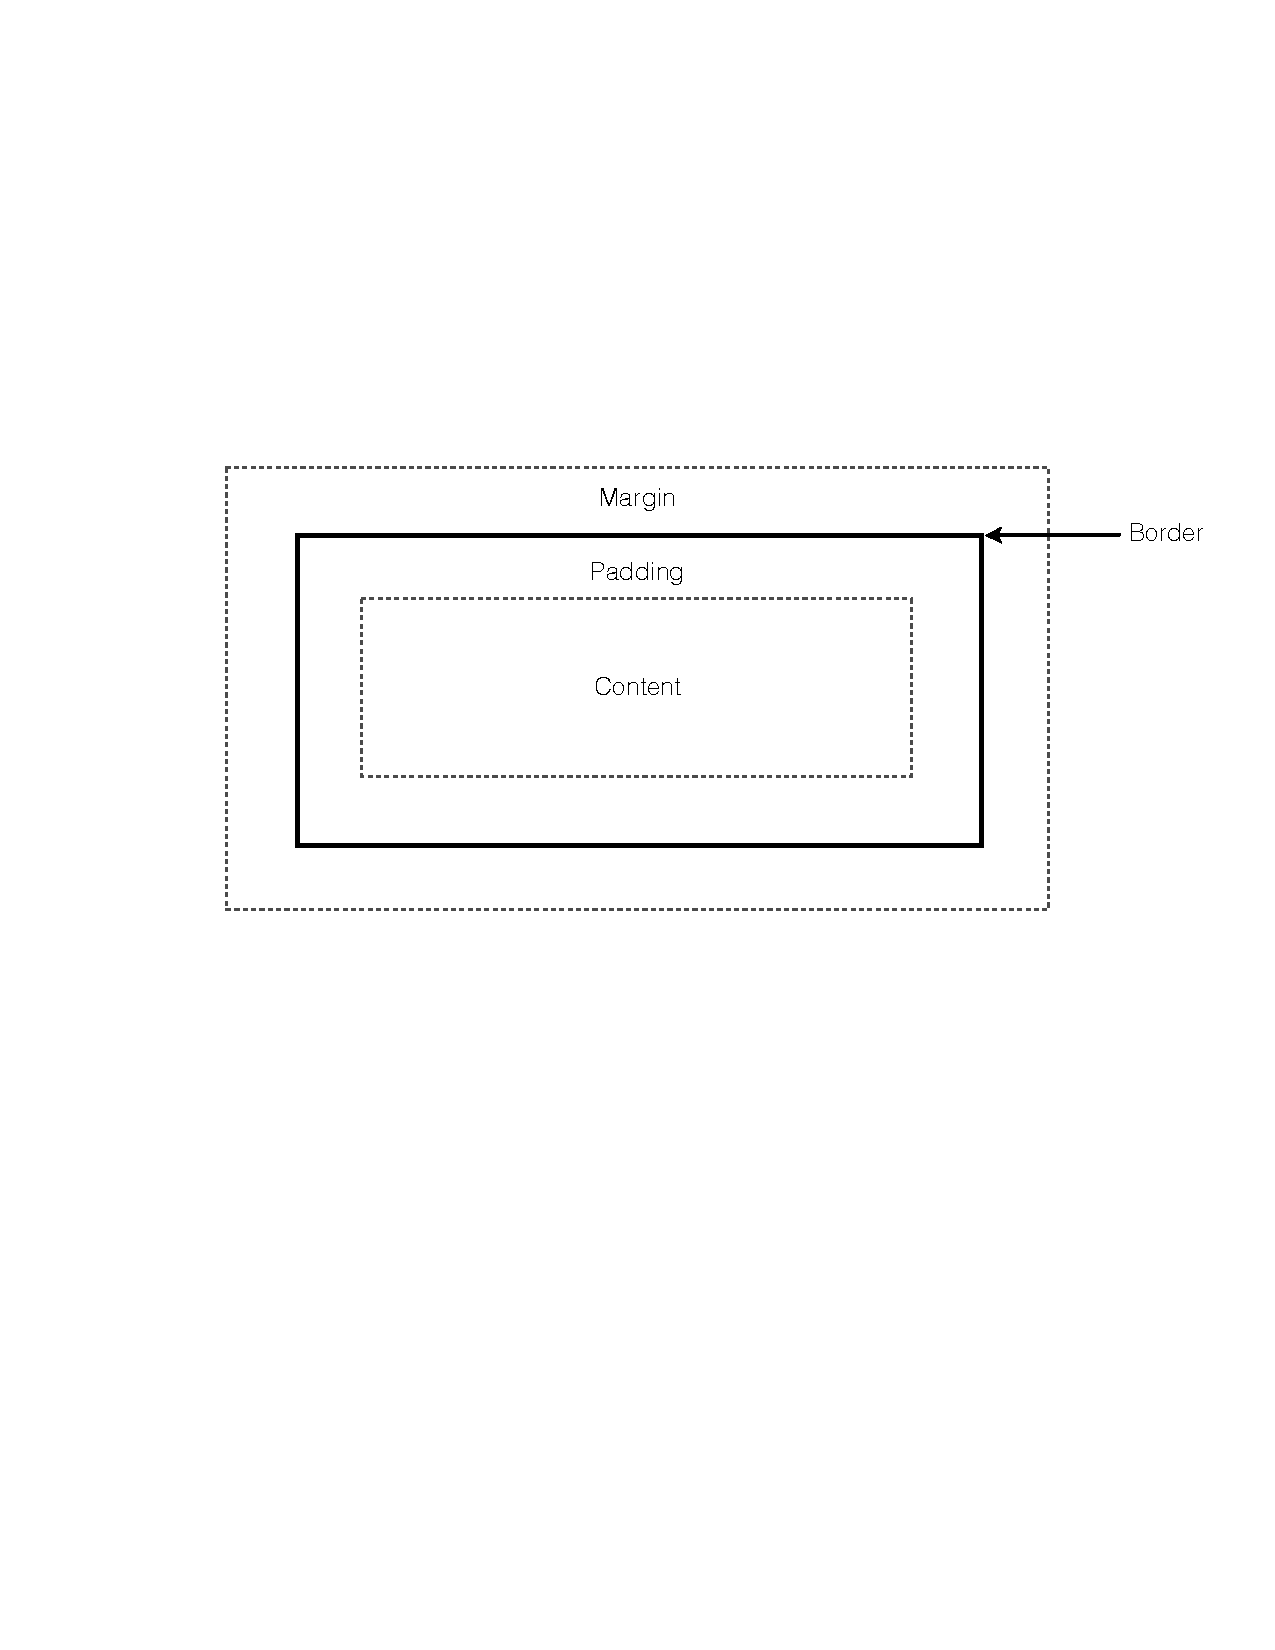
\includegraphics[width=\textwidth]{box_model}
	\caption{The Box Model}
	\label{fig:box_model}
\end{figure}

One should use \emph{margin} when spacing between elements is desired, and if one would like spacing from the content of the element to the border of the element, \emph{padding} should be used.





%----------------------------------------------------------------------------------------
%	CORE ELEMENTS
%----------------------------------------------------------------------------------------

\part{Core Elements}
%!TEX root = ../../main.tex

%!TEX root = ../../main.tex

\chapter{Icons}
\index{Icons}

Throughout the \giraf-software suite different icons will be used to reference different applications and functionalities. Refer to the sections below to see how and when to use these icons.

\section{\giraf Software Suite Icon}
\index{Icons}
The different applications in the \giraf software suite may want to refer to the software suite itself. To do this, the overall application icon seen in \figref{fig:overall_application_icon} can be used. This icon will also be used in some situations for indicating activity. \todo{Refer to a section describing activity indicators}

\begin{figure}[h]
	\centering
	
\includegraphics[scale=0.25]{placeholder}
	\caption{Overall application icon for the \giraf software suite}
	\label{fig:overall_application_icon}
\end{figure}

\section{Application-specific Icons}
\index{Icons}
Each application in the \giraf software suite must have its own icon. This icon should reflect the content and functionality of the application and must not be ambiguous. All application icons should furthermore use the icon-base seen in \figref{fig:application_specific_icon_base}. 
\\\\
Rendered icons must be available in sizes defined in the \href{http://developer.android.com/design/style/iconography.html}{Android Iconography article}. The foreground of the icon must be clear in any of these sizes. Furthermore, the icon must not appear smudged or otherwise distorted on any scale.

\begin{figure}[h]
	\centering
	
\includegraphics[width=0.15\textwidth]{application_specific_icon_base}
	\caption{Base for all application specific icon}
	\label{fig:application_specific_icon_base}
\end{figure}

\section{Icons used to represent functionality}
\index{Icons}
Specific icons may be used in buttons (See \texttt{GirafButton} in \gc) to represent functionality. The foreground of these icons must be gray-scaled and be quadratic (square). The functionality that the icon represents should be reflected in the icons itself. The icons should use the icon-base seen in \figref{fig:functionality_specific_icon_base}.

\begin{note}
	Please be aware that the actual icons should not be designed/rendered using the base as described above. Instead use the \texttt{GirafButton} from the \gc library. This will allow you to only design the actual foreground and not worry about the background (base).
\end{note}

\begin{figure}[h]
	\centering
	
\includegraphics[width=0.15\textwidth]{functionality_specific_icon_base}
	\caption{Base for all functionality-specific icons}
	\label{fig:functionality_specific_icon_base}
\end{figure}


%!TEX root = ../../main.tex

\chapter{Image Representation}
\index{Image}
\index{Pictogram}

For the following sections there exist a shared component called \androidinline{GirafPictogramItemView} which assists one to comply with the following design rules, for a guide on how to use this class see \appref{app:implementation_guide_for_pictures}.

\section{Appearance}
\label{sec:appearance}
In the \giraf software-suite there exist various types of images, such as pictograms and profile pictures. Images should be quadratic, have a white background (\colref{3.1}) regardless of content and have a black border (\colref{3.2}), as seen in \figref{fig:pictogram_image_view}. 

\begin{figure}[!htbp]
    \centering

    \begin{subfigure}[t]{0.4\textwidth}
    	\centering
        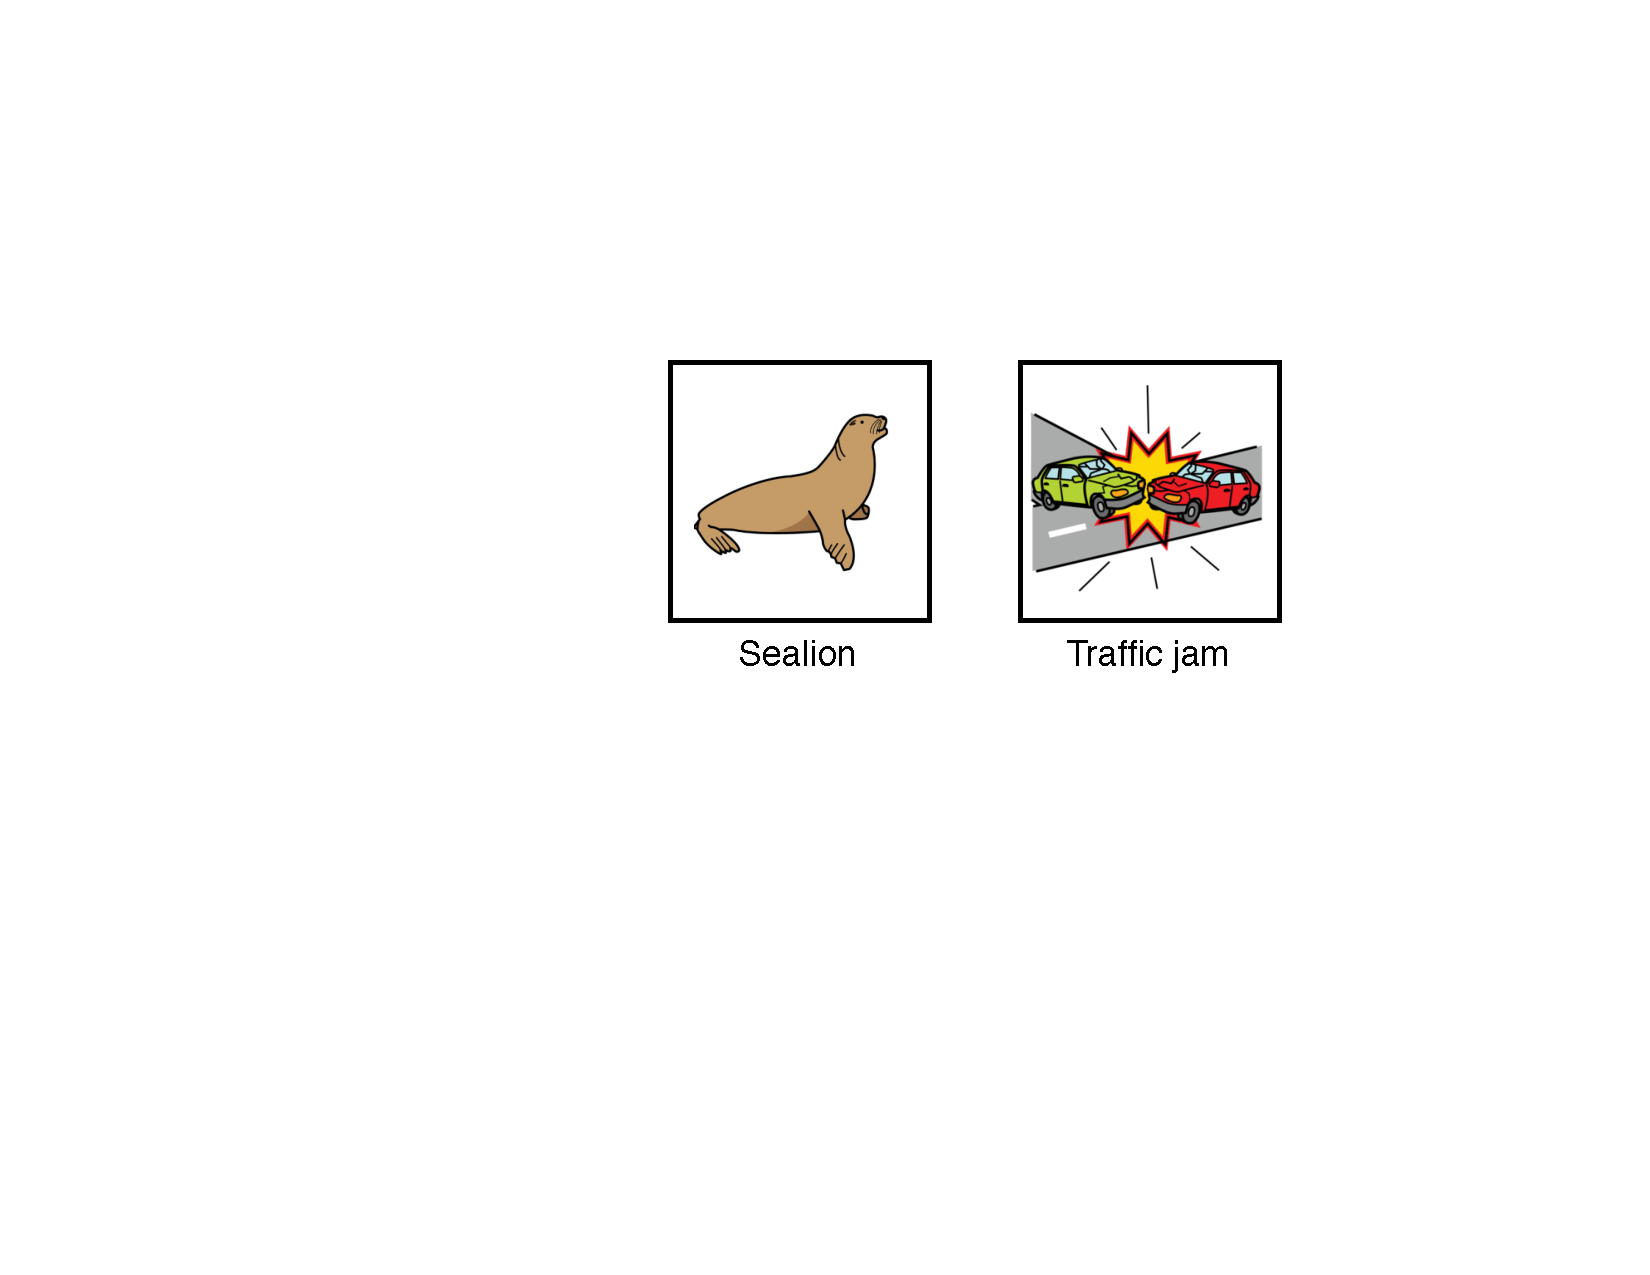
\includegraphics[scale=0.5]{pictogram_image_view_pictograms}
        \caption{Pictograms}
        \label{fig:pictogram_image_view_pictograms}
    \end{subfigure}
    \hspace{5em} 
    \begin{subfigure}[t]{0.4\textwidth}
    	\centering
        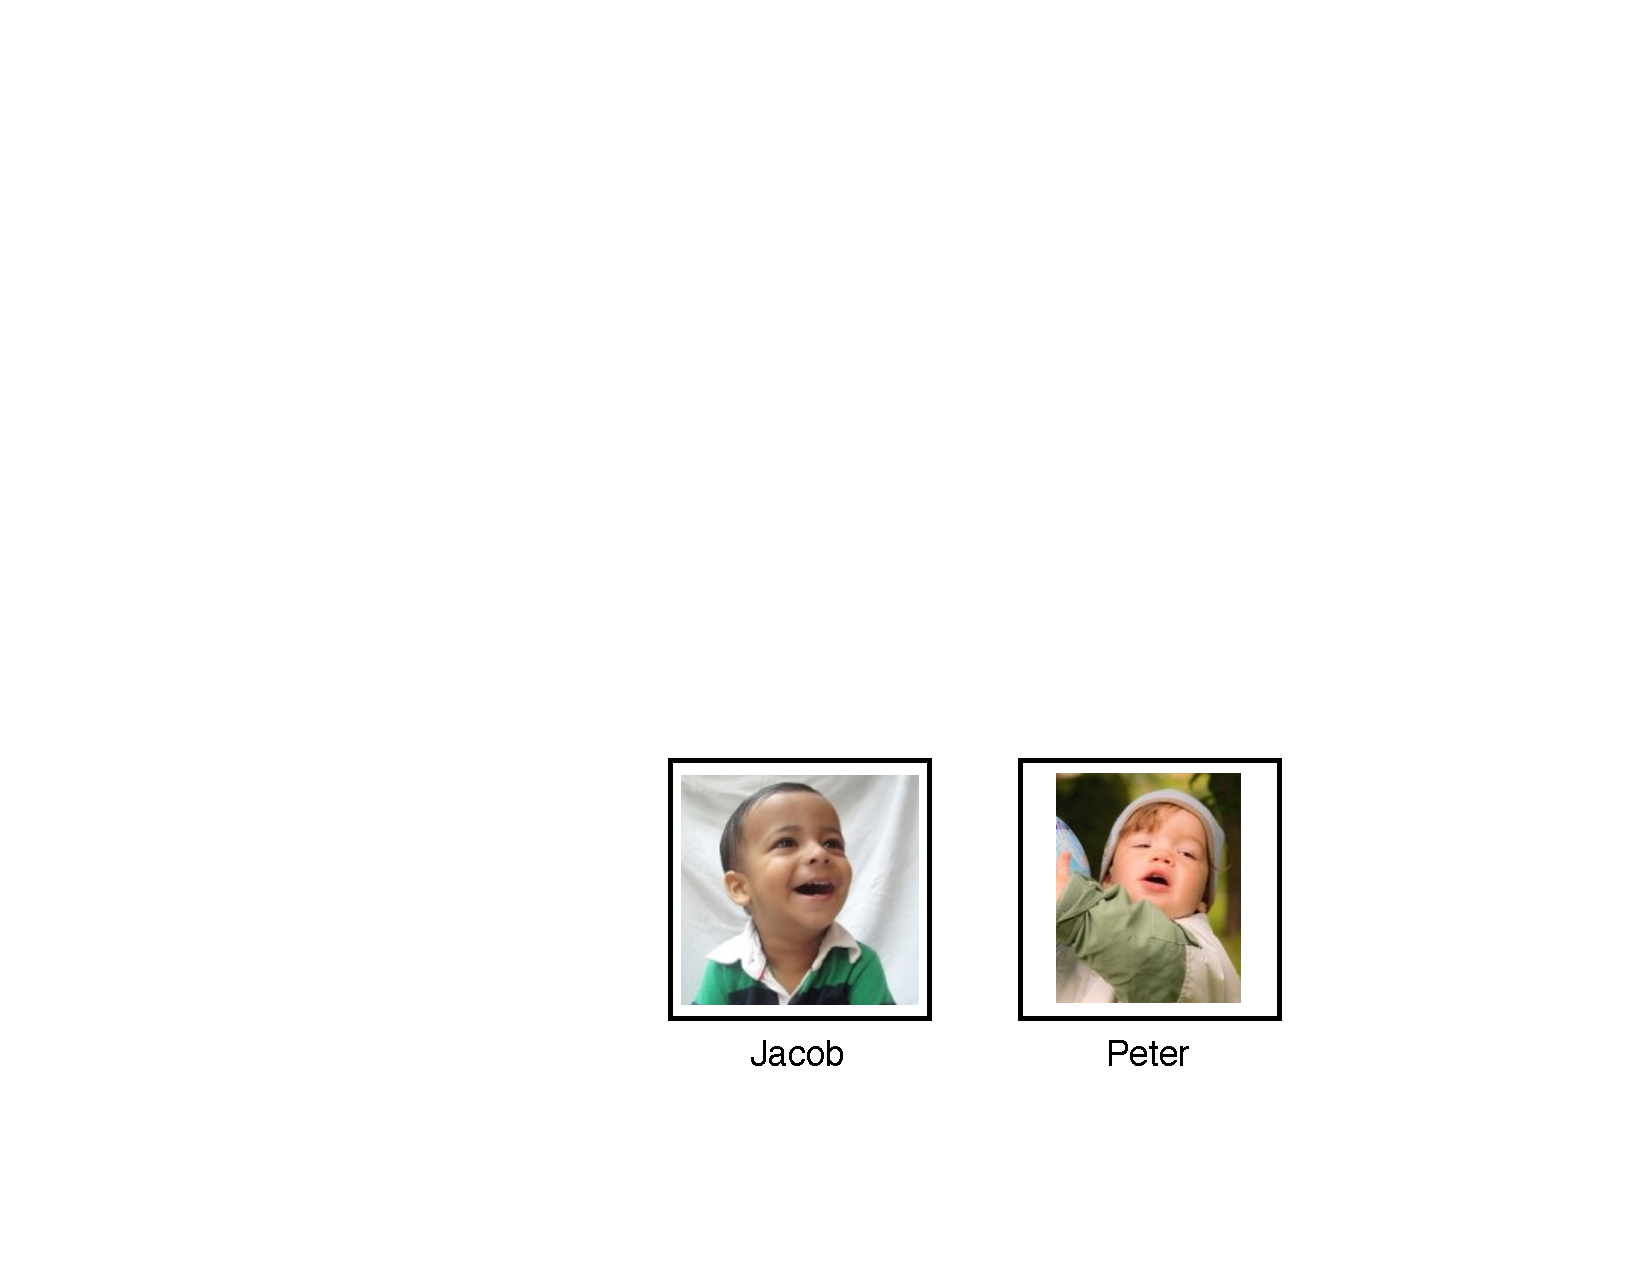
\includegraphics[scale=0.5]{pictogram_image_view_profiles}
        \caption{Profile pictures}
        \label{fig:pictogram_image_view_profiles}
    \end{subfigure}
    
    \caption{Image representation}
    \label{fig:pictogram_image_view}
\end{figure}

\begin{note}
	Profile pictures, as seen in \figref{fig:pictogram_image_view_profiles}, should, as the first profile (Jacob), fit to the canvas. However, many profile pictures are captured in a different way as seen in the second profile (Peter). It is wanted that in the future, when profile pictures are captured, that they only allow for pictures that have the layout of the first profile. For the sake of convenience and backwards compatibility we allow old profile pictures to be as the second.
\end{note}

\noindent
The image view should have a 10 dp padding so that the content gets spacing to the border as seen in \figref{fig:pictograms_padding}.

\begin{figure}[h]
	\centering
	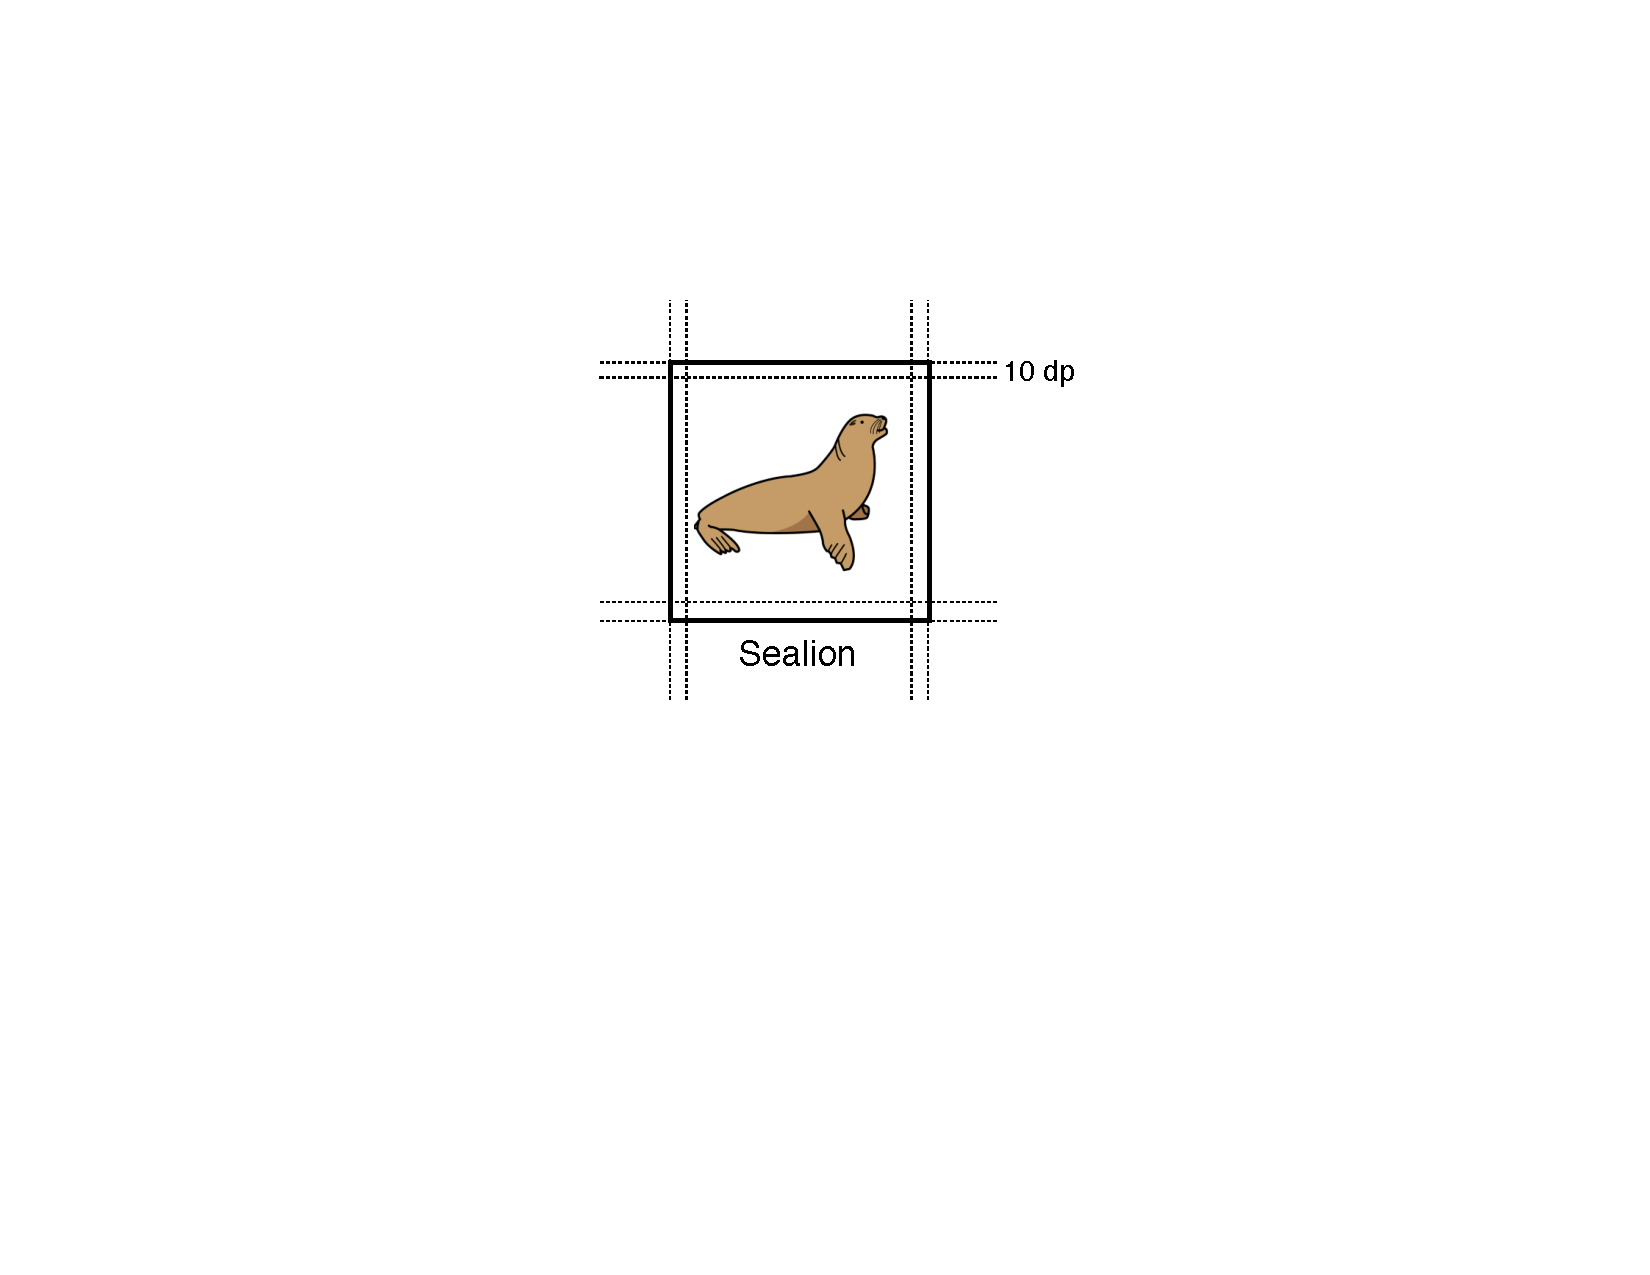
\includegraphics[width=0.35\textwidth]{pictograms_padding}
	\caption{Image representation}
	\label{fig:pictograms_padding}
\end{figure} 
\FloatBarrier

\subsection{Citizen view}
\label{sub:citizen_view}

When an image is present for a citizen it is not allowed for the image to be incomplete. See \figref{fig:citizen_image_view} for an example of how it should be shown to citizens and an example (\figref{fig:citizen_image_view_correct}) of how it should not be shown to citizens (\figref{fig:citizen_image_view_wrong}). 

\begin{figure}[!htbp]
    \centering

    \begin{subfigure}[t]{0.4\textwidth}
        \centering
        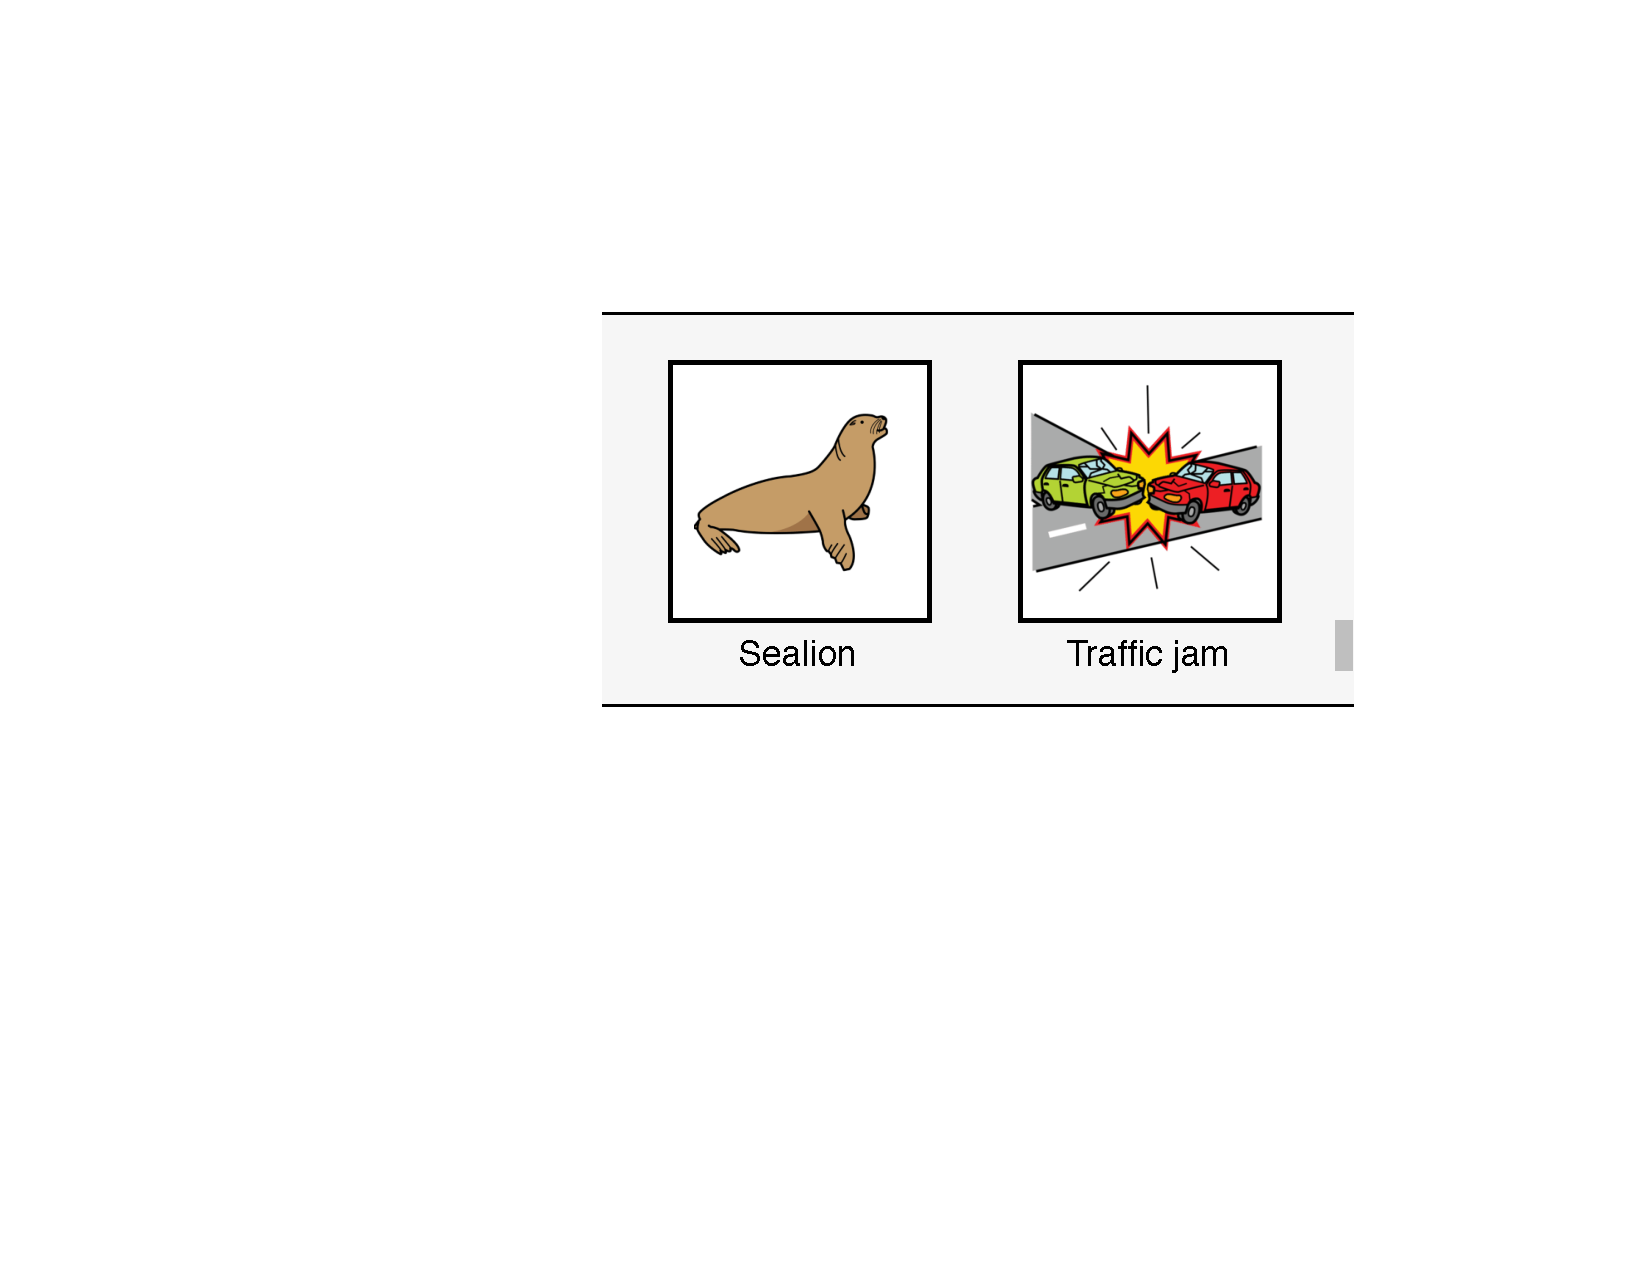
\includegraphics[scale=0.5]{citizen_view_correct}
        \caption{Correct citizen appearance}
        \label{fig:citizen_image_view_correct}
    \end{subfigure}
    \hspace{5em} 
    \begin{subfigure}[t]{0.4\textwidth}
        \centering
        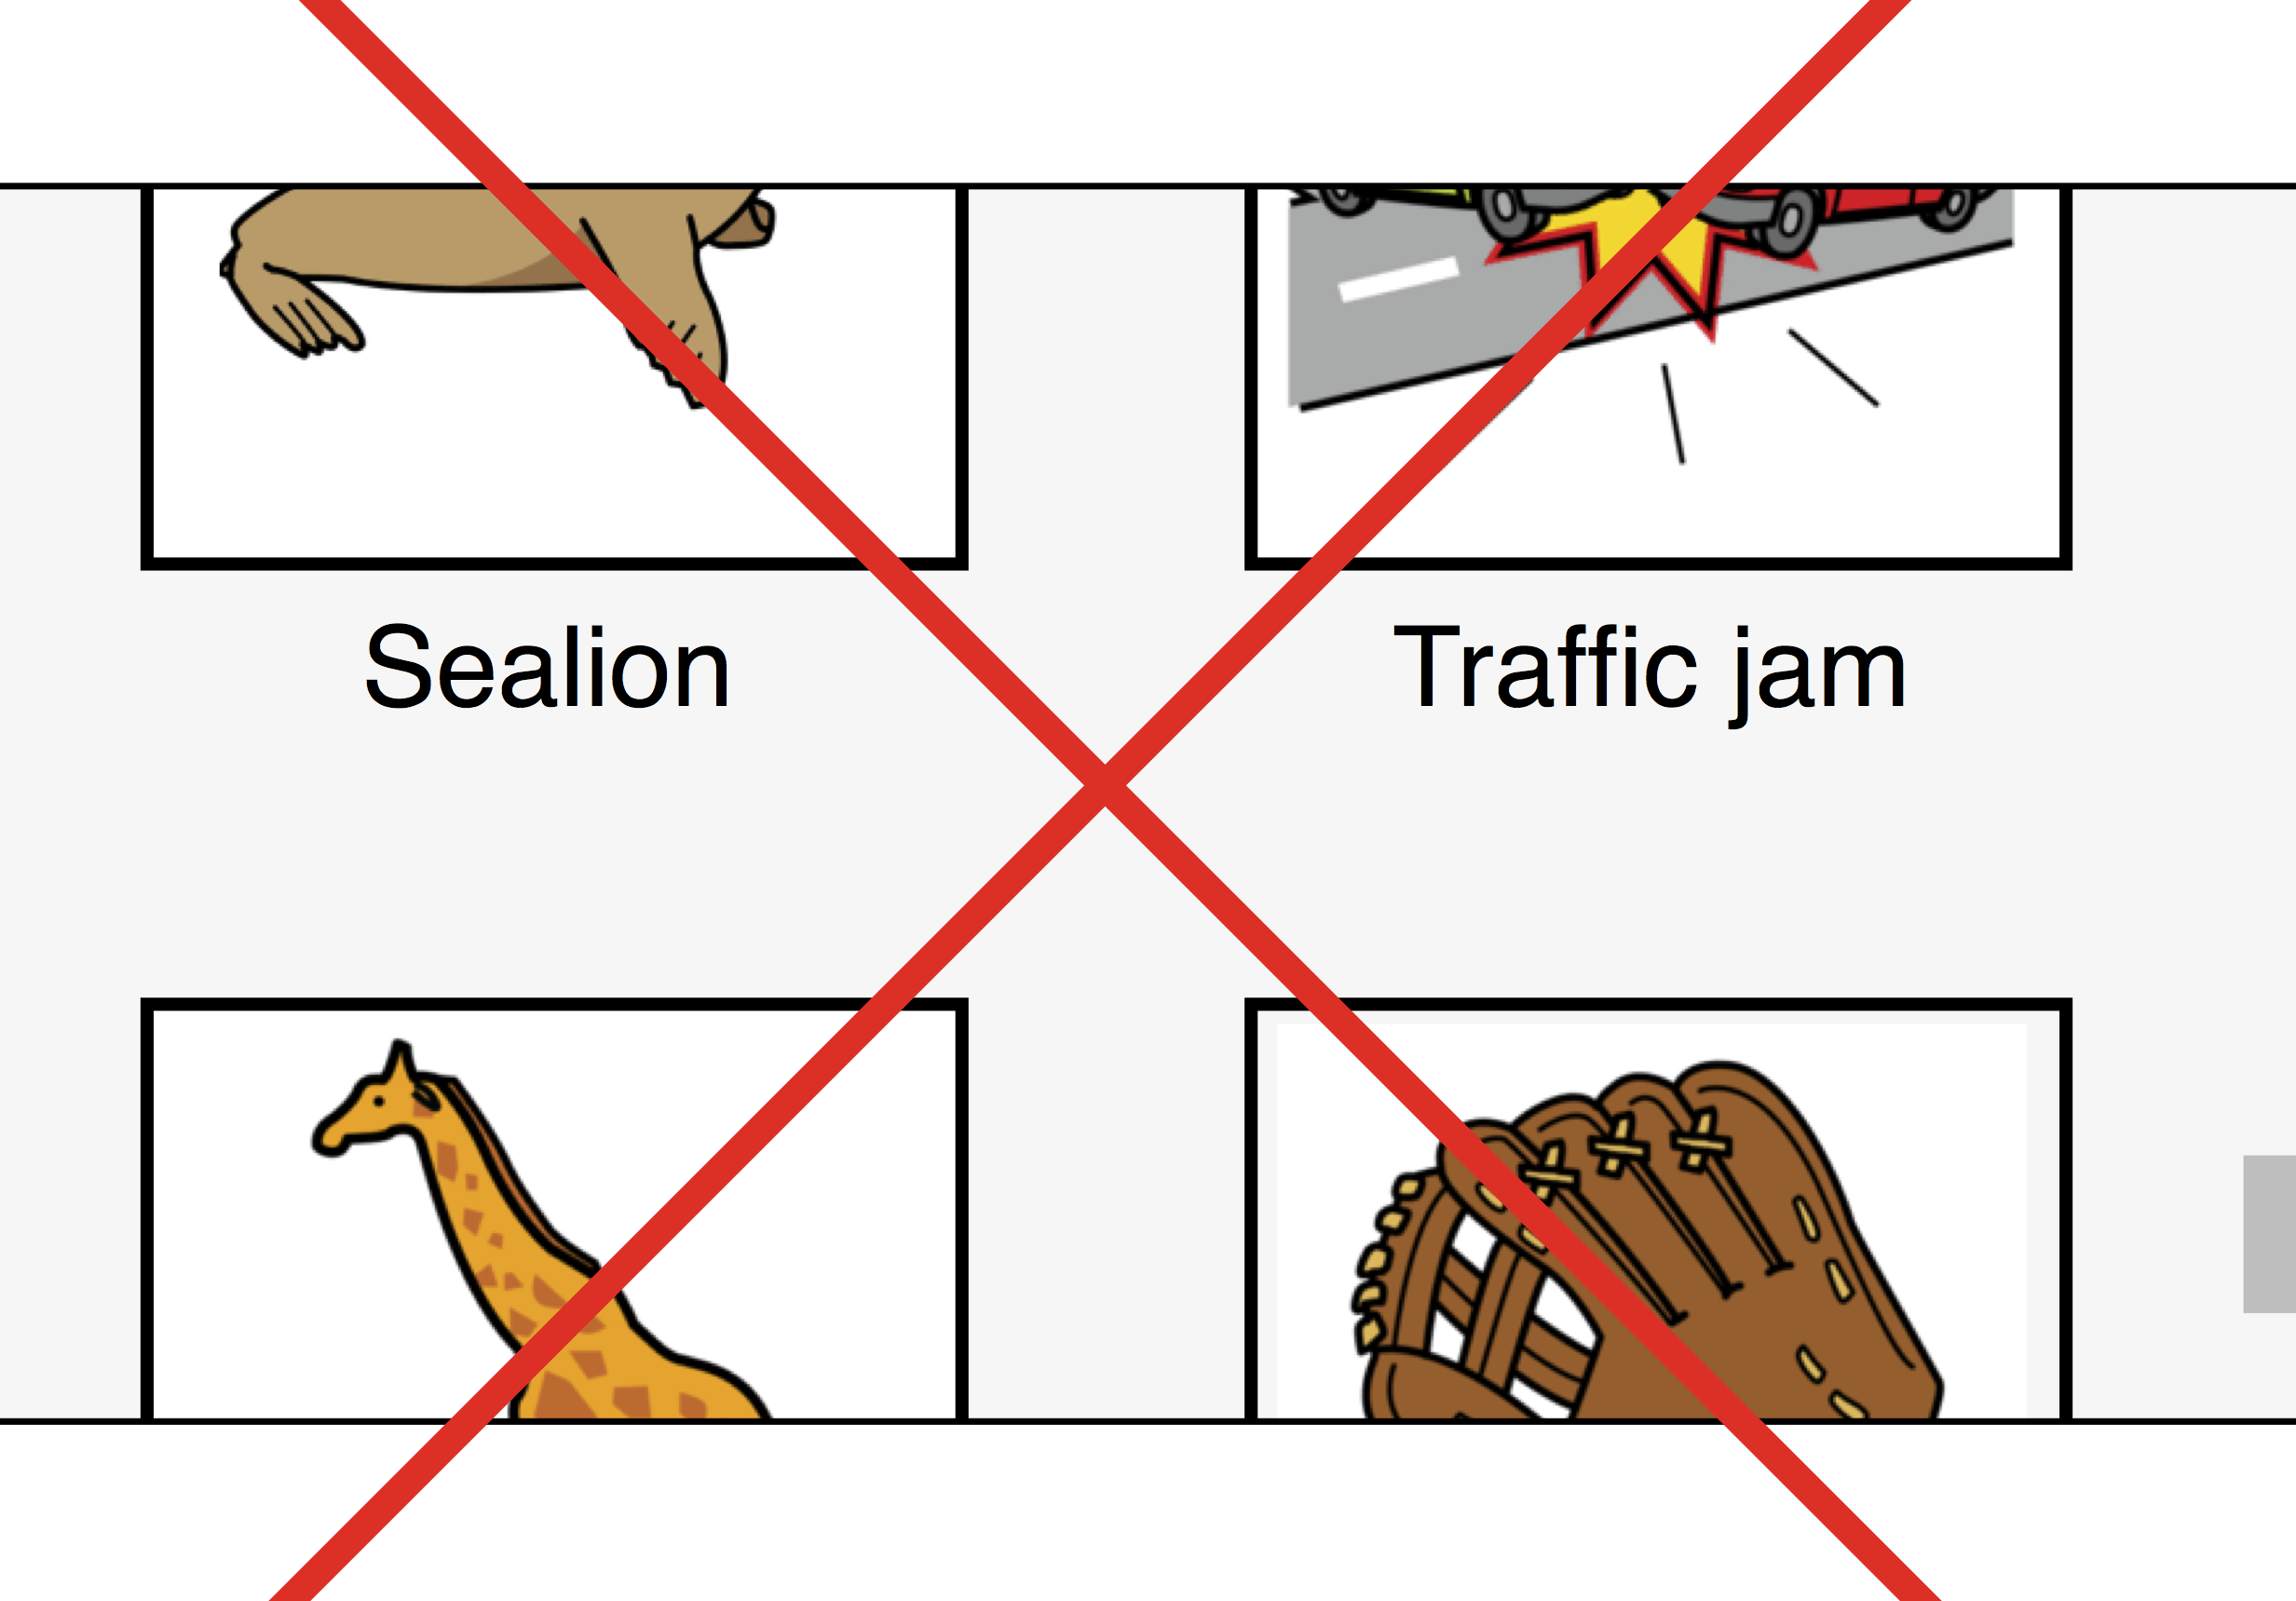
\includegraphics[scale=0.5]{citizen_view_wrong}
        \caption{Wrong citizen appearance}
        \label{fig:citizen_image_view_wrong}
    \end{subfigure}
    
    \caption{Citizen appearance explanation}
    \label{fig:citizen_image_view}
\end{figure}

\section{Marking}
\index{Marking}
\index{Selection}
\label{sec:marking}
It is often possible to mark images throughout the suite, and whenever this happens one should mark the background of the selected item with an orange color (\colref{3.3}), as seen in \figref{fig:pictograms_marked}. 

\begin{figure}[!htbp]
    \centering

    \begin{subfigure}[t]{0.4\textwidth}
    	\centering
        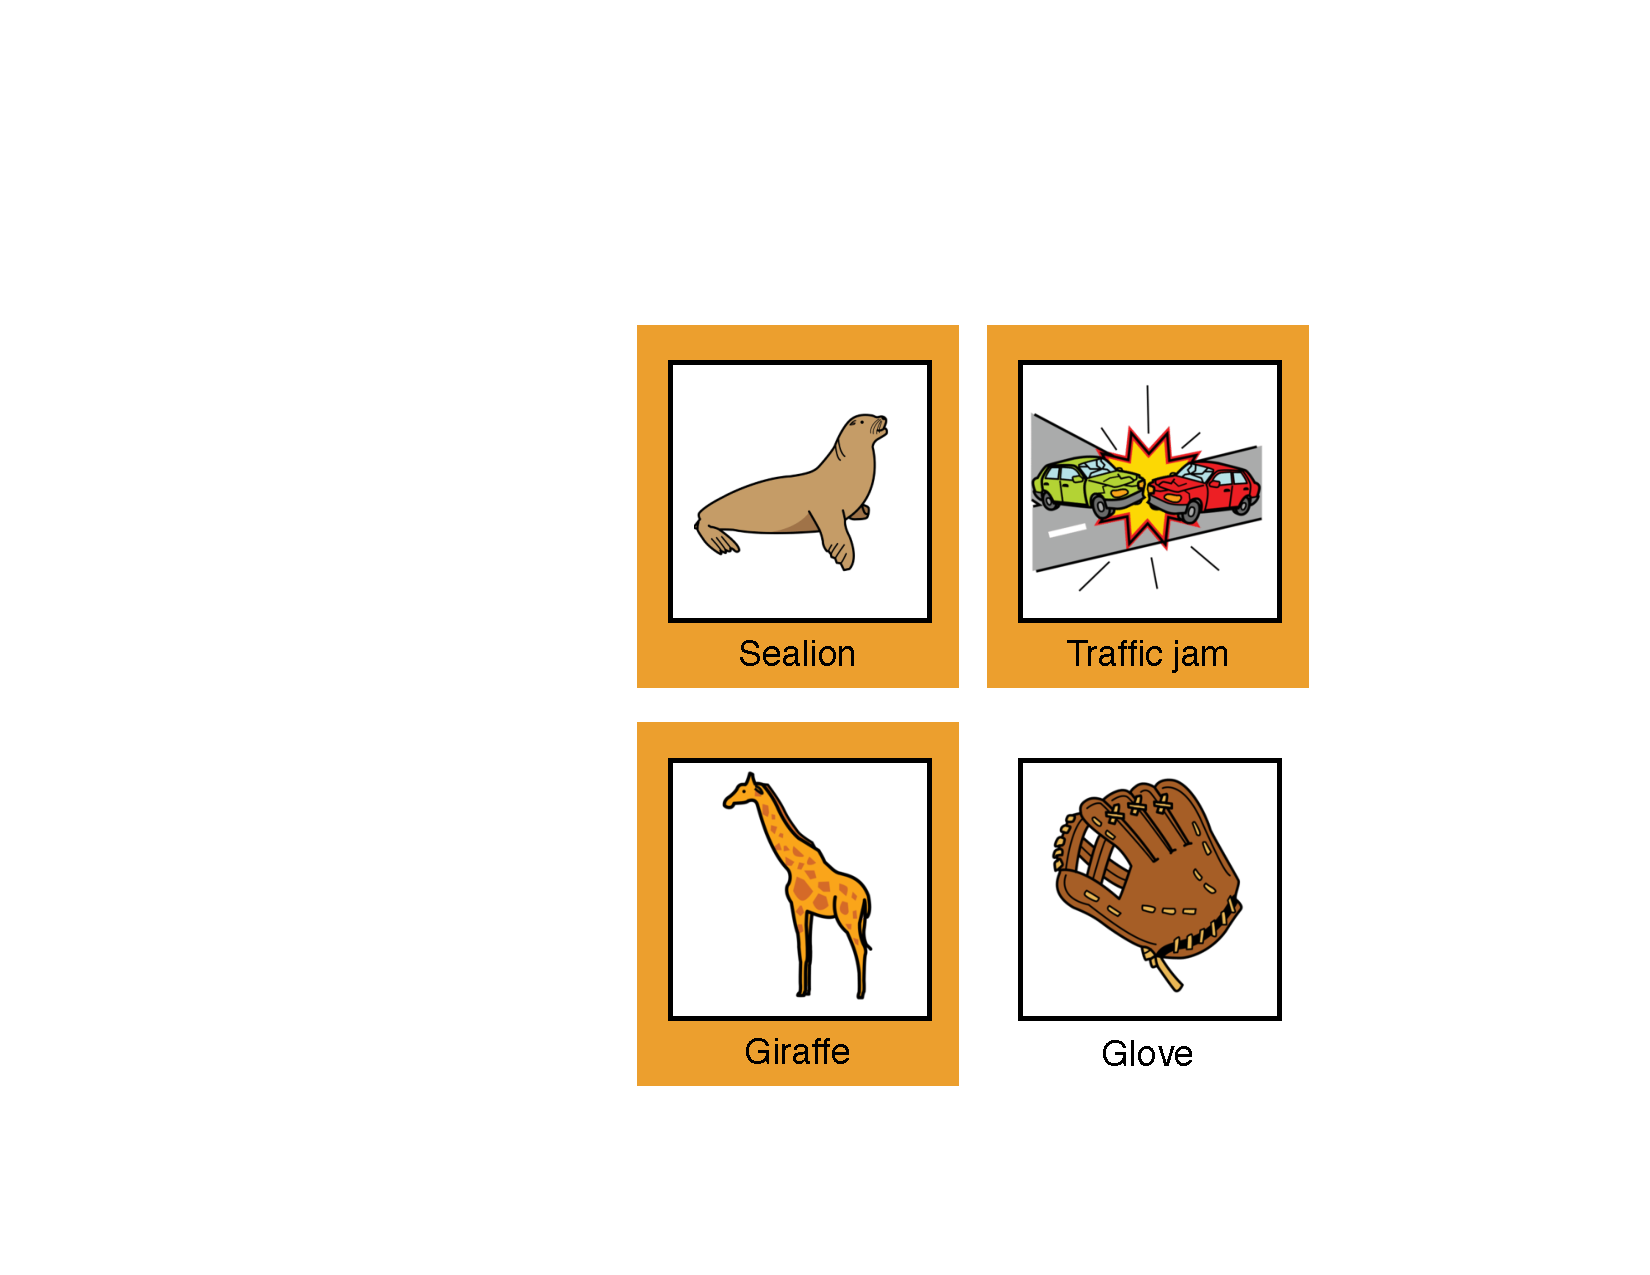
\includegraphics[scale=0.5]{pictograms_marked_correct}
        \caption{Corrected marking}
        \label{fig:pictograms_marked_corect}
    \end{subfigure}
    \hspace{5em} 
    \begin{subfigure}[t]{0.4\textwidth}
    	\centering
        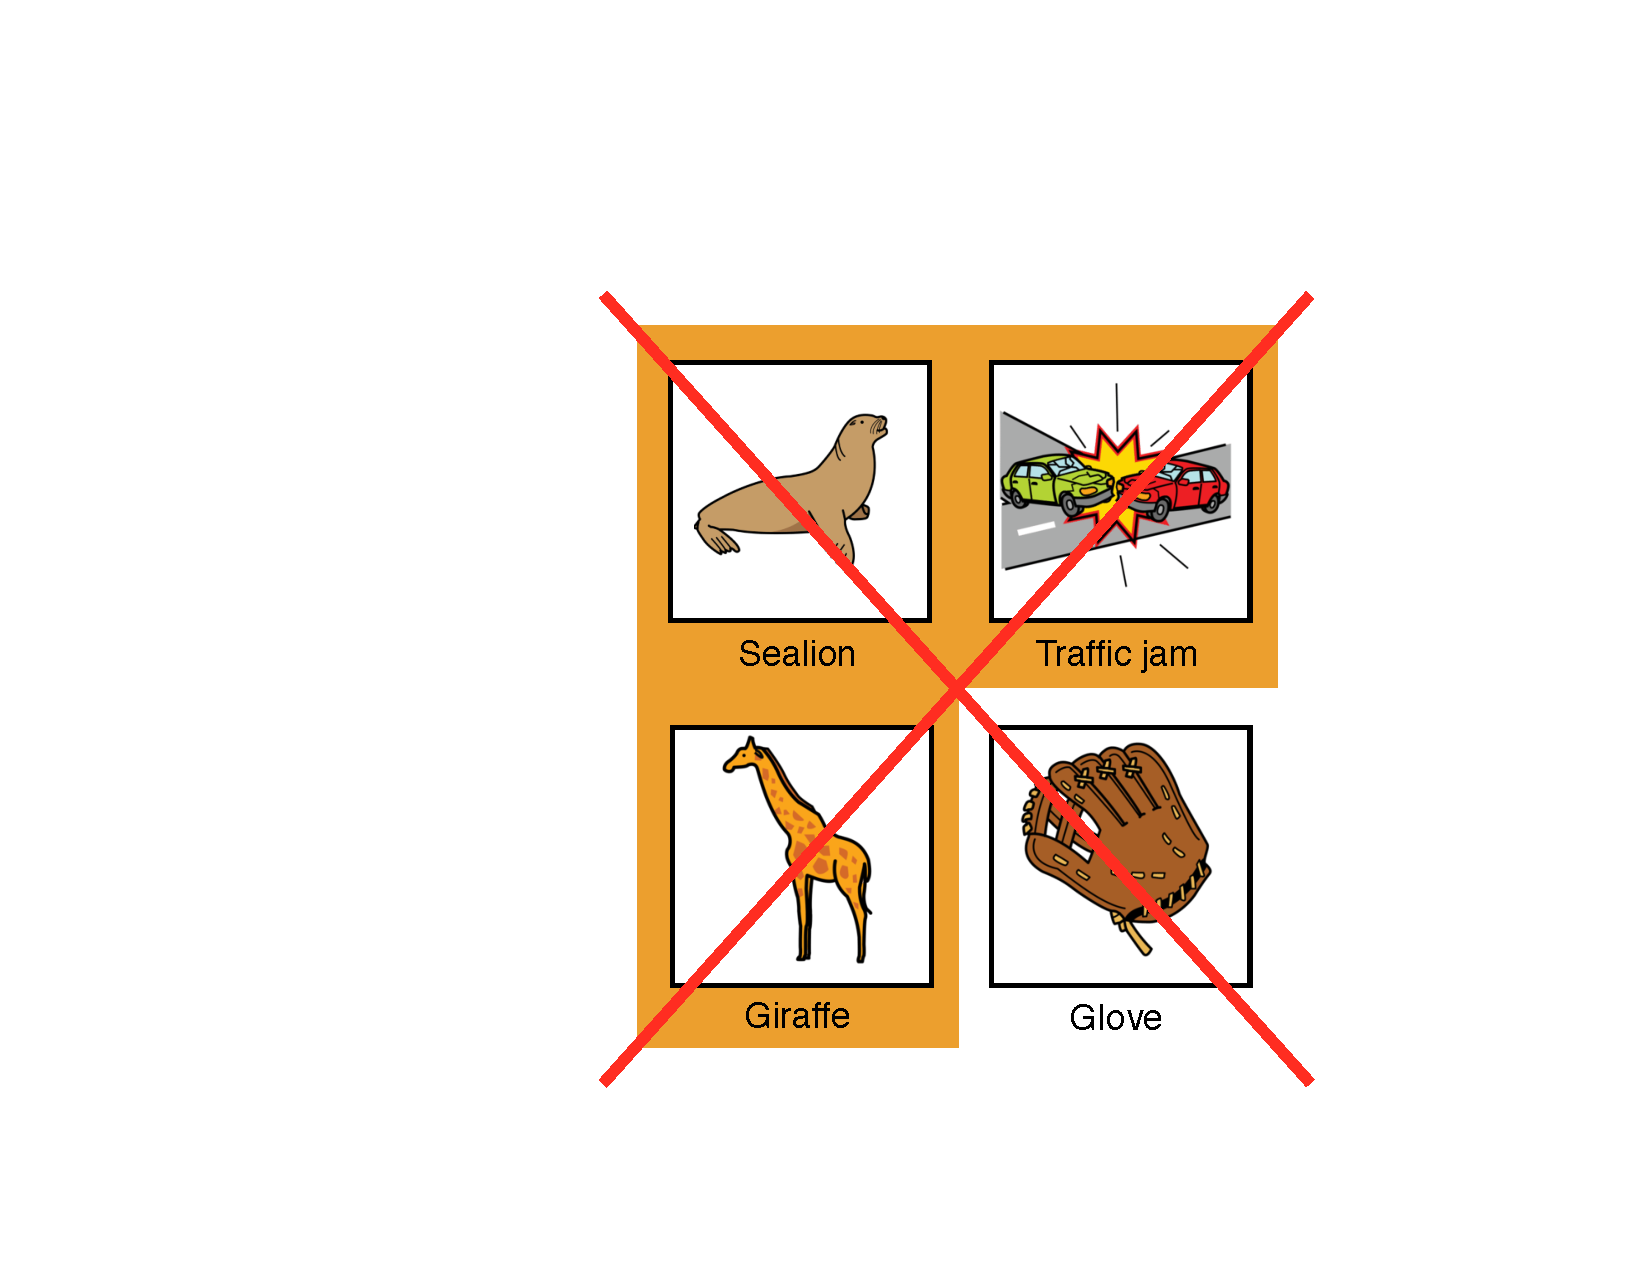
\includegraphics[scale=0.5]{pictograms_marked_wrong}
        \caption{Wrong marking}
        \label{fig:pictograms_marked_wrong}
    \end{subfigure}
    
    \caption{Marking of images}
    \label{fig:pictograms_marked}
\end{figure}

\begin{note}
	It is important that when having multiple marked images that there are some margin between these elements. This should be implemented as seen in \figref{fig:pictograms_marked_corect}, and not as seen in \figref{fig:pictograms_marked_wrong}.
\end{note} 

\section{Indicator overlay}
\index{Overlay}
\index{Overlay!Custom indicator}
\index{Overlay!Editable indicator}
\index{Indicator}
\index{Indicator!Editable indicator}
\index{Indicator!Custom indicator}
\index{Editable}
\label{sec:indicator_overlay}

If one wants to indicate that an image is editable, for instance when picking an icon for a category, the image should have an overlay indicating this as seen in \figref{fig:pictogram_indicator_overlay_editable}. Other types of indicators should look similar, e.g. when indicating that an image is a placeholder for a category it is indicated as seen in \figref{fig:pictogram_indicator_overlay_category}.

\begin{figure}[!htbp]
    \centering

    \begin{subfigure}[t]{0.4\textwidth}
        \centering
        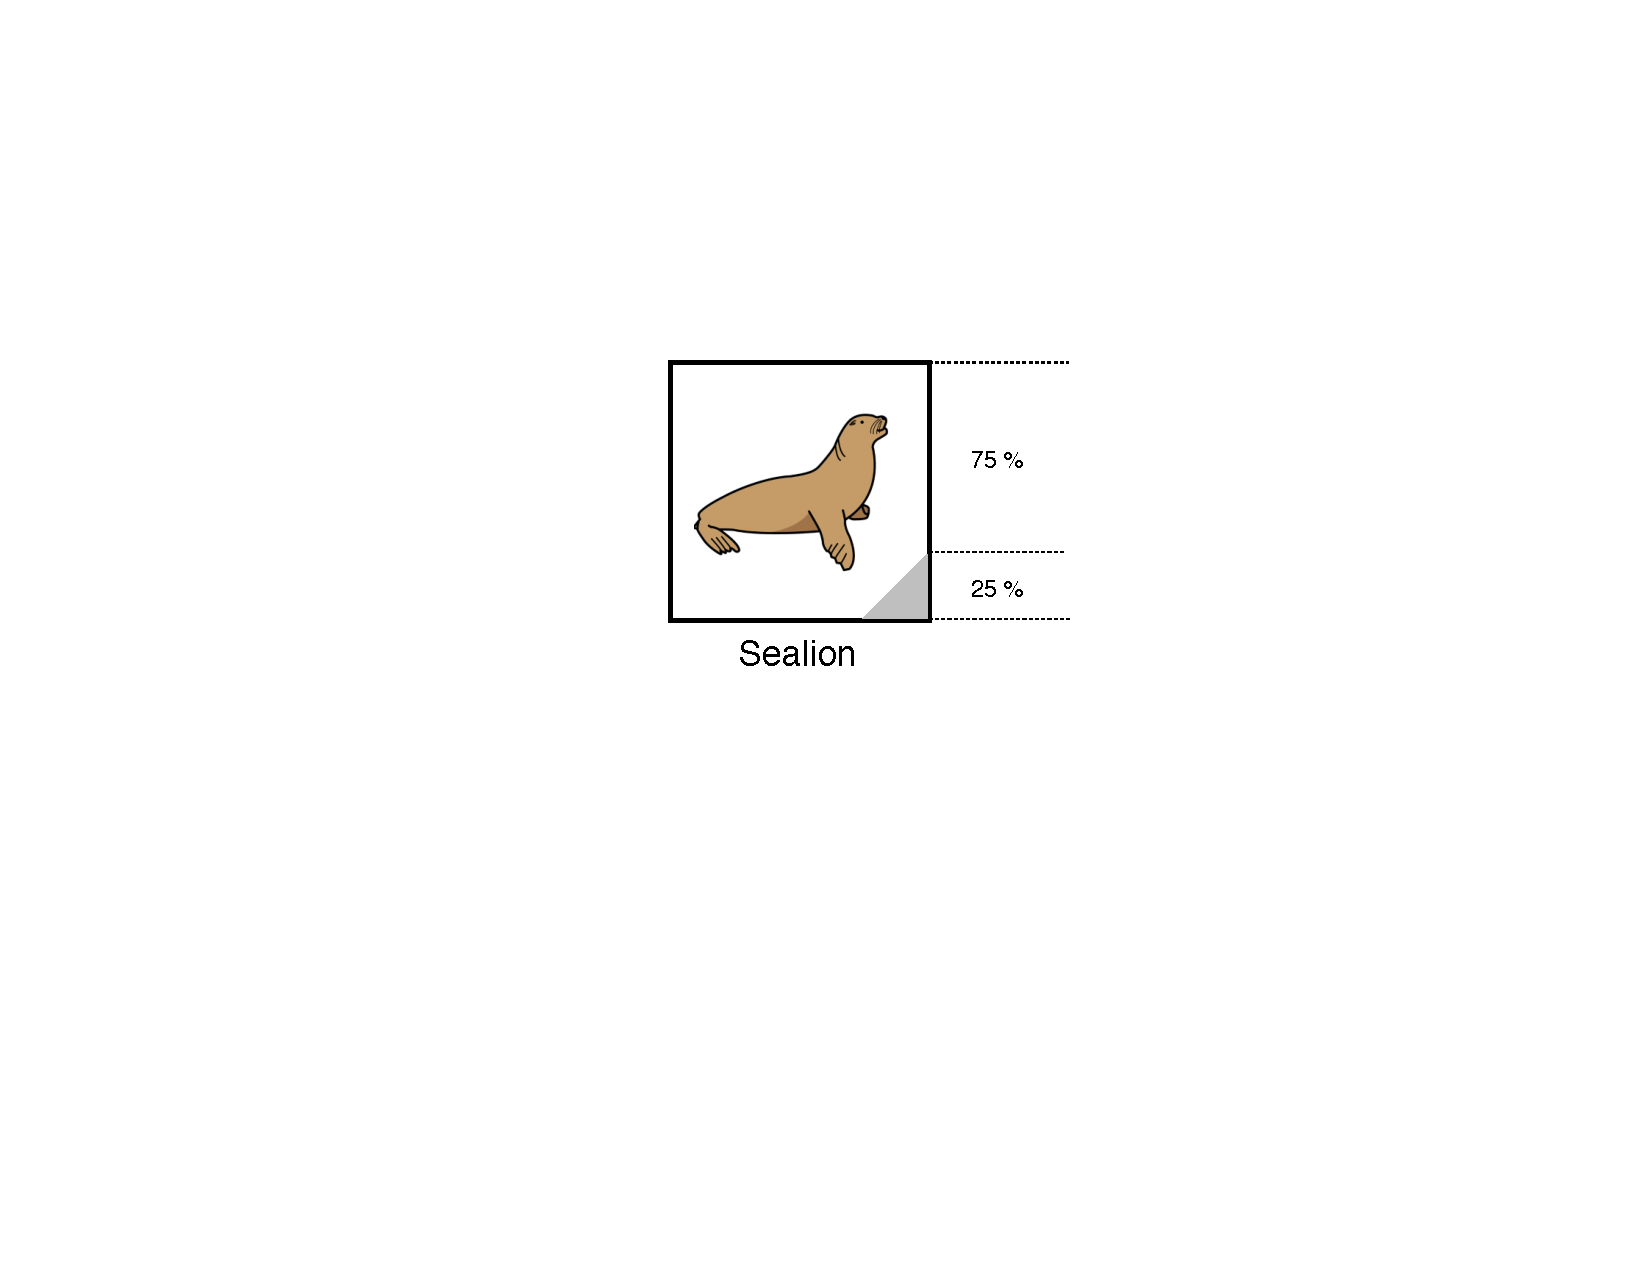
\includegraphics[scale=0.6]{pictogram_indicator_overlay_editable}
        \caption{Editable indicator}
        \label{fig:pictogram_indicator_overlay_editable}
    \end{subfigure}
    \hspace{5em} 
    \begin{subfigure}[t]{0.4\textwidth}
        \centering
        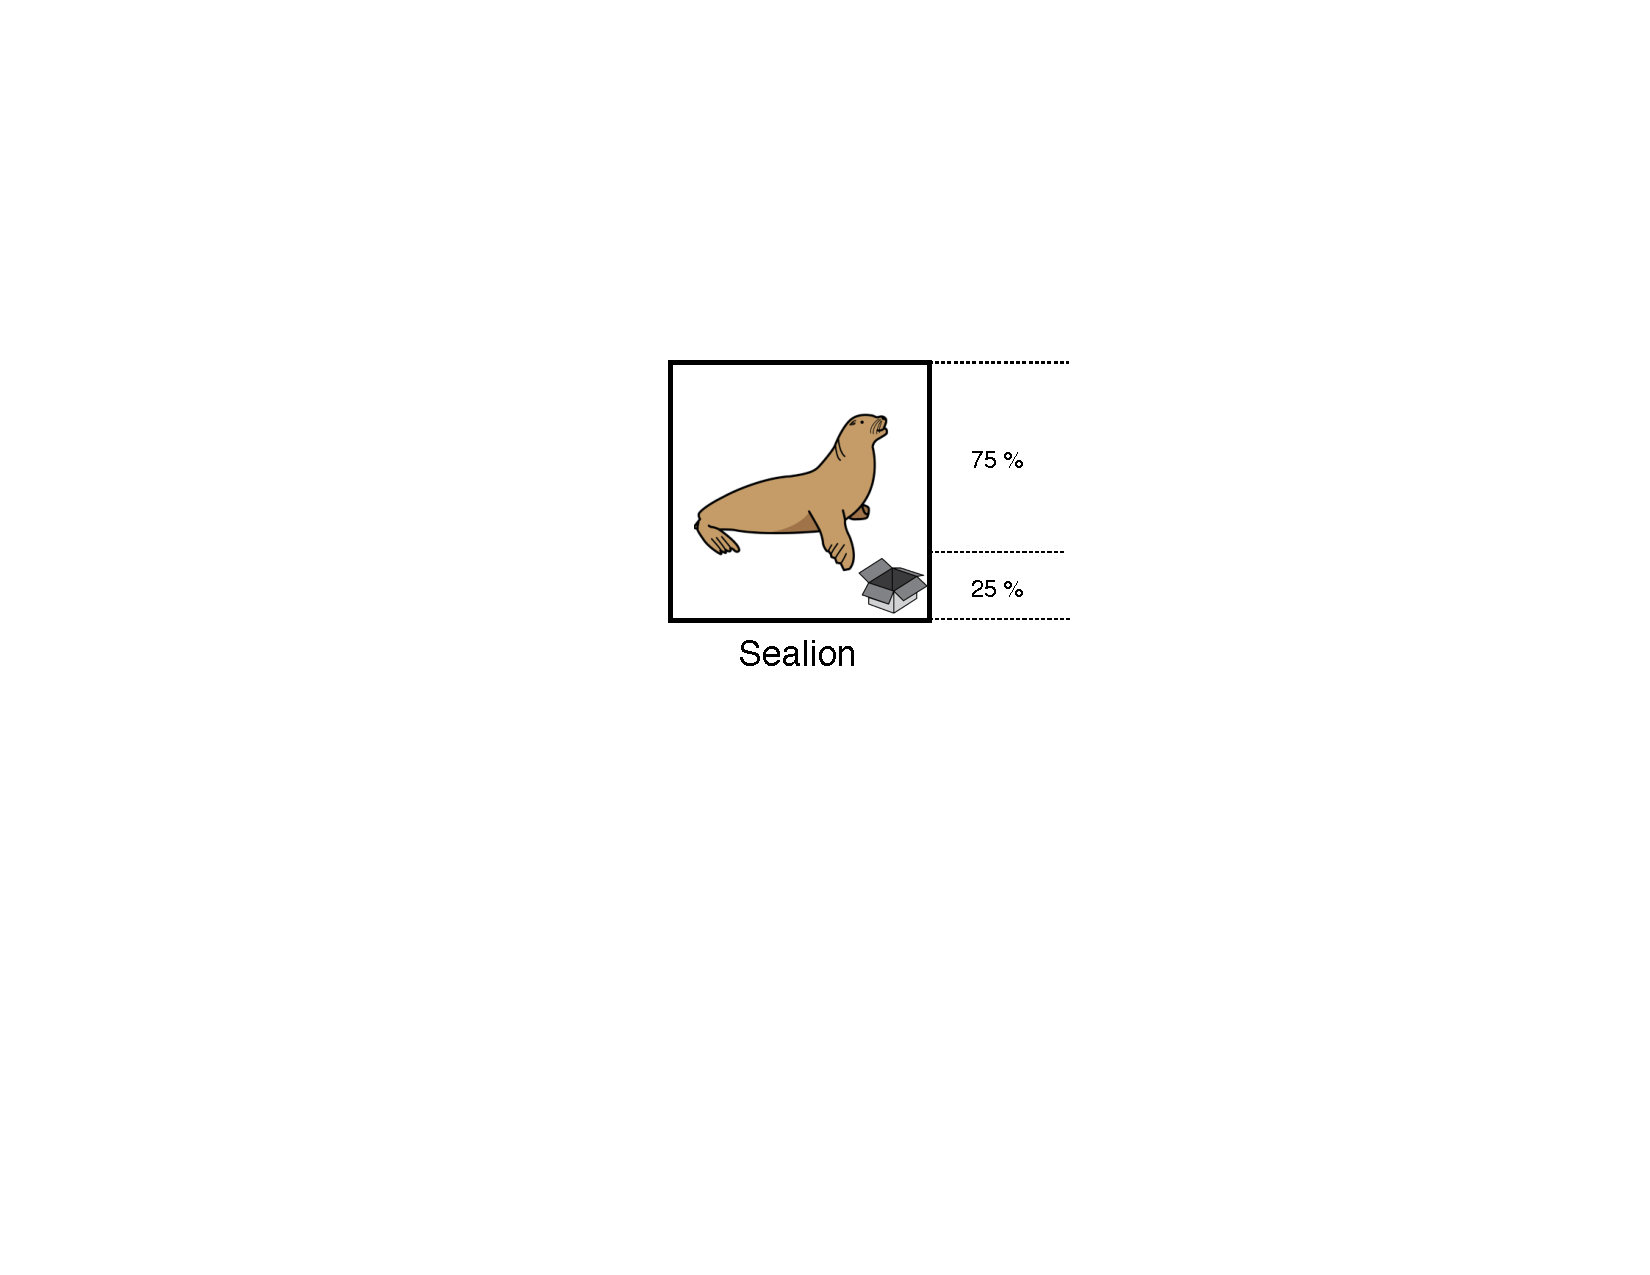
\includegraphics[scale=0.6]{pictogram_indicator_overlay_category}
        \caption{Category indicator}
        \label{fig:pictogram_indicator_overlay_category}
    \end{subfigure}
    
    \caption{Indicator overlays}
    \label{fig:pictograms_overlay}
\end{figure}


%!TEX root = ../../main.tex

\chapter{Typography}
% TODO: Write about the typography

\section{Fonts, Sizes and Colors}
When creating text fields in the \giraf software suite, is it imperative that they look alike across the entire suite. For this reason one should at all times use the default font-type in the applications. \\

\noindent The size of any text across the applications should always be given in ``SP'', and should always be readable on both 7 and 10 inch tablets. It is up to the developers of the individual applications to decide upon a specific text-size, but it should fit the general layout of the suite. \\

\noindent All text should by default be black (\#000000) across the suite when placed in buttons, views, etc. When creating hint text, e.g. when there are no applications present in the launcher, one should use the android implementation of Darker Gray\footnote{http://developer.android.com/reference/android/R.color.html\#darker\_gray}. When using the showcase library to highlight features, the text color of the help text should be white (\#FFFFFF), so it is readable on the dark background. 

%!TEX root = ../../main.tex

\chapter{Tone of Voice}
\index{Tone of voice}
\index{Voice}
When displaying messages to the user the following rules must be respected.

\section{Short and Precise}
All messages must be short and precise. If a part of a sentence is redundant, remove it. However, you must provide enough information to cover the whole situation.

\begin{exampleR}[Correct use]
	The application can only be started from a guardian profile
\end{exampleR}

\begin{exampleW}[Incorrect use]
	The application could not be started
\end{exampleW}

\begin{exampleW}[Incorrect use]
	The application could not be started unless you start it from a guardian profile. Please log onto a guardian profile to gain access to this application.
\end{exampleW}

\section{Addressing Users}
When referring to people with Autism Spectrum Disorder (ASD), use the word \textit{citizens}. When referring to either institutional- or legal guardians, use the word \textit{guardian}.

\begin{exampleR}[Correct use]
	The application cannot be started from a citizen-profile
\end{exampleR}

\begin{exampleW}[Incorrect use]
	The application cannot be started from a child-profile
\end{exampleW}

%!TEX root = ../../main.tex

\chapter{Application structure}
% TODO: Describe a generic application and how it should be structured. For instance the use of the topbar or sidemenu. Also talk about contextual menus.

\section{Top Bar}
\index{Action bar}
\index{Top bar}
An Android \androidinline{Activity} includes an optional top bar which if utilized should look like \figref{fig:top_bar_example}. A top bar should have the standard top bar size in Android.\\
The top bar should only include buttons related to the entire Activity and should not depend on the context inside the activity.

\begin{note}
Such a top bar is easily achieved by letting your \androidinline{Activity} extend the \androidinline{GirafActivity} from the Giraf Components library.
\end{note}

\begin{figure}[!htbp]
        \centering
        
\includegraphics[width=0.75\textwidth]{pictures/application_structure/topbar}
        \caption{Top bar example}
        \label{fig:top_bar_example}
\end{figure}

\FloatBarrier


\section{Side Bar}
\index{Side bar}

Side bars need not, but may be contextual. It is recommended to use side bars to switch between content of applications. A side bar should look like \figref{fig:side_bar_example}.

\begin{figure}[!htbp]
        \centering
        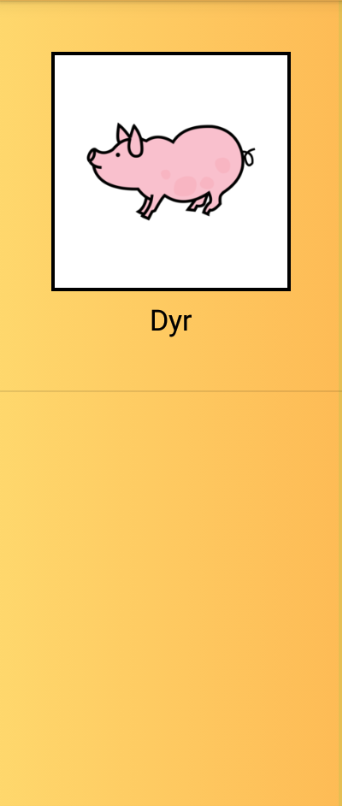
\includegraphics[width=0.25\textwidth]{pictures/application_structure/sidebar}
        \caption{Side bar example}
        \label{fig:side_bar_example}
\end{figure}

\FloatBarrier


\section{Bottom bar}
\index{Bottom bar}
Bottom bars should be entirely contextual and depend on the current content displayed in the current \androidinline{Activity}. A bottom bar should look like \figref{fig:bottom_bar_example}.

\begin{figure}[!htbp]
        \centering
        
\includegraphics[width=0.75\textwidth]{pictures/application_structure/bottombar}
        \caption{Bottom bar example}
        \label{fig:bottom_bar_example}
\end{figure}

\FloatBarrier


\section{Content}
The main content of applications should be in the center of the layout and any menu bars should be above, under, and to the sides of the main content. 

\begin{note}
We recommend using Android \androidinline{Fragment} instances to manage content of an \androidinline{Activity} if the main content of an Android \androidinline{Activity} needs to change between different content that needs to be controlled differently. 
\end{note}


\section{Clickable Elements}
All elements that are clickable must have a safety-distance to other elements. This will ensure that the user does not accidentally press the wrong thing and ultimately does something wrong. This safety distance may be achieved using several different methods. Please refer to the following sections. \figref{fig:correct_element_spacing} shows an example of correct item spacing while \figref{fig:incorrect_element_spacing} shows an example of incorrect item spacing.
\\\\
Elements must have a safety distance to \ldots
\index{Margin}
\begin{itemize}
        \item Other clickable elements
        \item Borders of it's container
        \item Borders of the tablet
\end{itemize}

\begin{figure}[!htbp]
    \centering
    \begin{subfigure}[t]{0.4\textwidth}
        \centering
        
\includegraphics[scale=0.1]{correct_element_spacing}
        \caption{Correct item spacing}
        \label{fig:correct_element_spacing}
    \end{subfigure}
    \hspace{5em} 
    \begin{subfigure}[t]{0.4\textwidth}
        \centering
        
\includegraphics[scale=0.1]{incorrect_element_spacing}
        \caption{Incorrect item spacing}
        \label{fig:incorrect_element_spacing}
    \end{subfigure}
    
    \caption{Examples of correct and incorrect element spacing}
    \label{fig:element_spacing_examples}
\end{figure}

\subsection{Element Margin}
\index{Margin}
Elements may be spaced apart from each other using margin on the individual elements. The distance between the elements should be consistent throughout all activities of any given application. \figref{fig:element_margin_example} shows an example of the margin for a given element.. 

\begin{figure}[h]
        \centering
        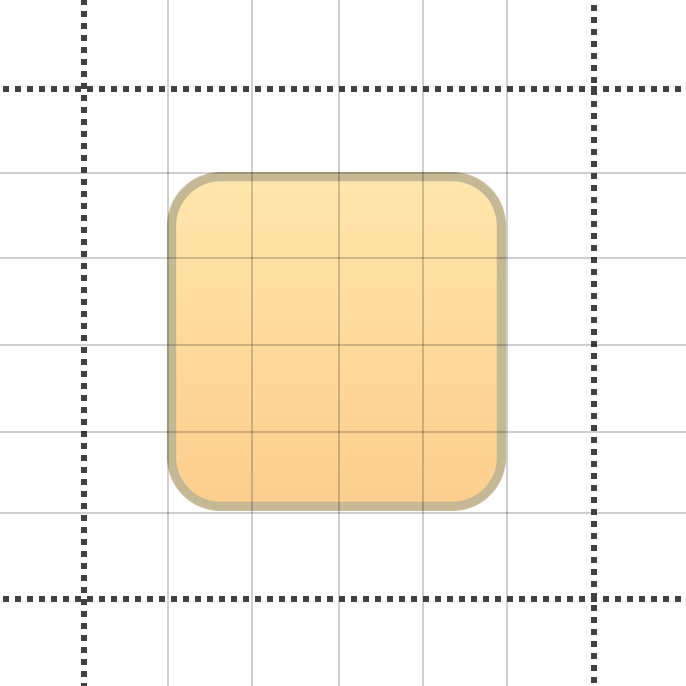
\includegraphics[width=0.25\textwidth]{element_margin_example}
        \caption{Example of element margin}
        \label{fig:element_margin_example}
\end{figure}

\begin{note}
        If margin is used inside a container each element with margin will also be a certain distance from the borders of that specific container. If, for instance, an element has a margin of $10$, then this element would be a distance of $10$ from the borders of the container. This means that there \textit{might} not be need for any padding on the given container.
\end{note}

\subsubsection{Consistent Margin}
\index{Margin}
Elements of the same type appearing in the same context must have the same distance to other elements. However, if the elements appear in an order, for example a horizontal list, the first and last element may differ. For instance, the first element may have a smaller left-margin and the last element may have a smaller right-margin. \figref{fig:element_margin_consistency} shows an illustration of this example.

\begin{figure}[h]
        \centering
        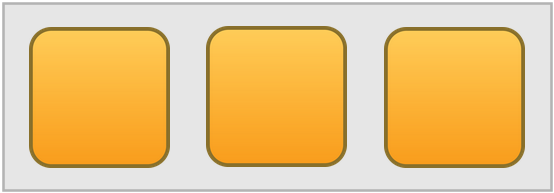
\includegraphics[width=0.45\textwidth]{element_margin_consistency}
        \caption{Example of element margin}
        \label{fig:element_margin_consistency}
\end{figure}


\subsection{Container Padding}
\index{Padding}
Each container should provide some padding for its content. This padding should be somewhat identical to the spacing between elements inside the container. \figref{fig:container_padding_example} shows an example of a container with padding. 

\begin{figure}[h]
        \centering
        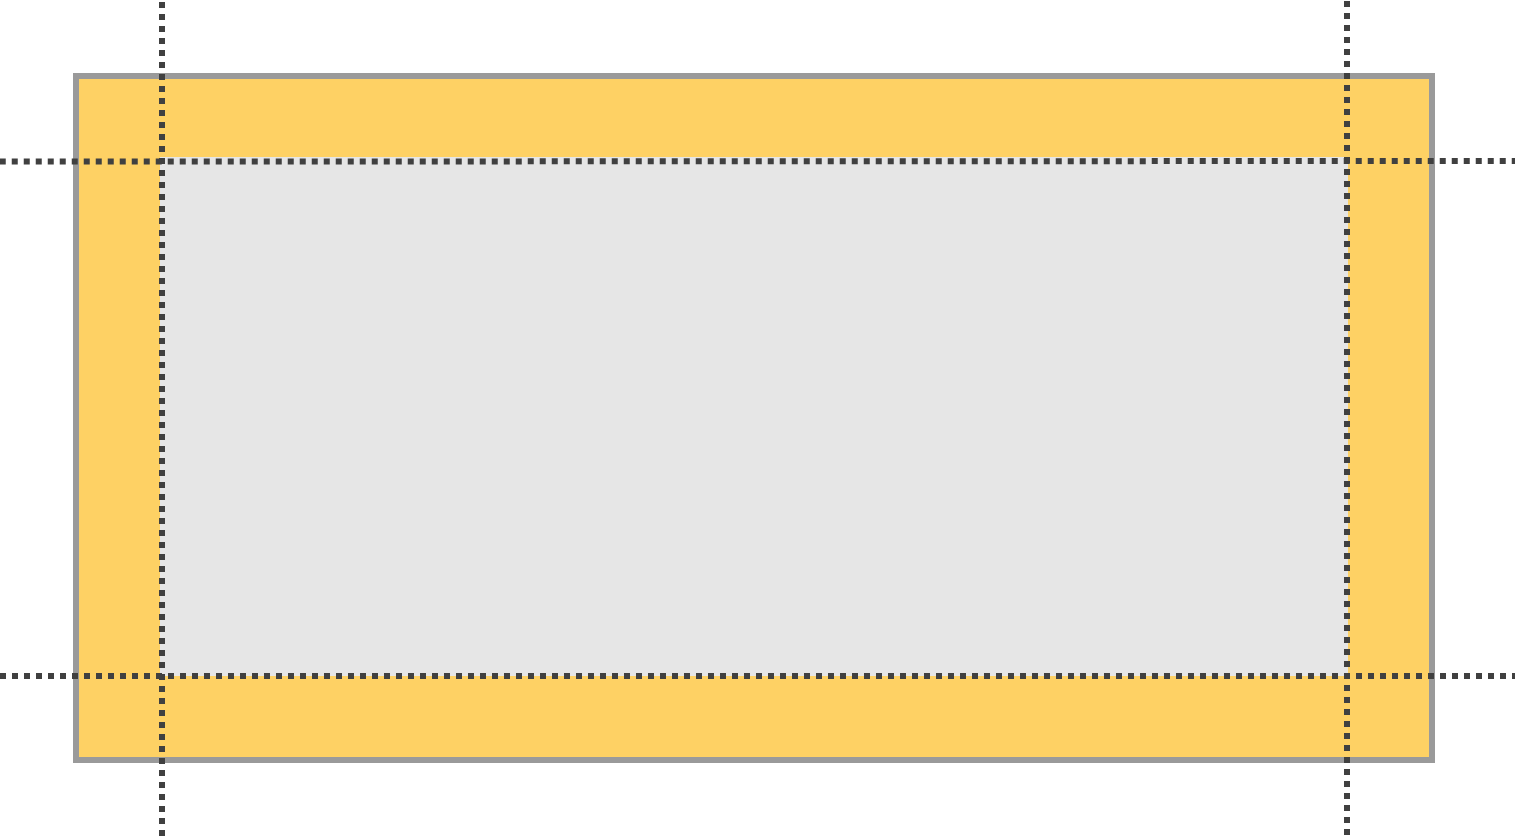
\includegraphics[width=0.65\textwidth]{container_padding_example}
        \caption{Example of a container with padding}
        \label{fig:container_padding_example}
\end{figure}

\begin{note}
        Whenever the content of the container can be scrolled through (for example a \texttt{GridView}) a property called \texttt{clipToPadding} must be set to \texttt{false}. Please refer to the \href{http://developer.android.com/reference/android/view/ViewGroup.html#attr_android:clipToPadding}{Android documentation} for additional information.
\end{note}\todo{The effect of this could be explained more clearly using a figure}


%!TEX root = ../../main.tex

\chapter{Colors}
\index{Colors}
Throughout this chapter a single color in each entry will denote a solid color, while two colors in an entry will denote a gradient between the two colors.

\section{Text and Background}
\index{Colors!Text color}
\index{Colors!Background color}
These colors should be used throughout any application.

\begin{table}[!htbp]
	\begin{tabularx}{\textwidth}{c X r c}
		\collabel{1.1}
		& Regular text-color 
		& \texttt{\#000000} & \cellcolor[HTML]{000000}\phantom{--} \\ \hline
	\end{tabularx}
\end{table}

\begin{table}[!htbp]
	\begin{tabularx}{\textwidth}{c X r c}
		\collabel{1.2}
		& Text-color used to indicate placeholder or hint-texts 
		& \texttt{\#AAAAAA} & \cellcolor[HTML]{AAAAAA}\phantom{--} \\ \hline
	\end{tabularx}
\end{table}

\begin{table}[!htbp]
	\begin{tabularx}{\textwidth}{c X r c}
		\collabel{1.3}
		& Background-color for any applications window background 
		& \texttt{\#000000} & \cellcolor[HTML]{000000}\phantom{--} \\ \hline
	\end{tabularx}
\end{table}

\begin{table}[!htbp]
	\begin{tabularx}{\textwidth}{c X r c}
		\collabel{1.4}
		& Background-color for any activity 
		& \texttt{\#E9E9E9} & \cellcolor[HTML]{E9E9E9}\phantom{--} \\ \hline
	\end{tabularx}
\end{table}

\section{Buttons}
\index{Colors!Button colors}
All buttons in the \giraf software suite should use these colors for buttons. Please note that all gradients defined below are from top to bottom. Also note that the colors for the disabled button must be slightly transparent ($65\%$).

\begin{table}[!htbp]
	\begin{tabularx}{\textwidth}{c X r c r c}
		\collabel{2.1}
		& Regular button background 
		& \texttt{\#FFCD59} & \cellcolor[HTML]{FFCD59}\phantom{--}
		& \texttt{\#FF9D00} & \cellcolor[HTML]{FF9D00}\phantom{--} \\ \hline
	\end{tabularx}
\end{table}

\begin{table}[!htbp]
	\begin{tabularx}{\textwidth}{c X r c r c}
		\collabel{2.2}
		& Regular button stroke/border 
		& ~ & ~
		& \texttt{\#8A6E00} & \cellcolor[HTML]{8A6E00}\phantom{--} \\ \hline
	\end{tabularx}
\end{table}

\begin{table}[!htbp]
	\begin{tabularx}{\textwidth}{c X r c r c}
		\collabel{2.2}
		& Pressed button background 
		& \texttt{\#D4AD2F} & \cellcolor[HTML]{D4AD2F}\phantom{--}
		& \texttt{\#FF9D00} & \cellcolor[HTML]{FF9D00}\phantom{--} \\ \hline
	\end{tabularx}
\end{table}

\begin{table}[!htbp]
	\begin{tabularx}{\textwidth}{c X r c r c}
		\collabel{2.3}
		Pressed button stroke/border 
		& ~ & ~
		& \texttt{\#493700} & \cellcolor[HTML]{493700}\phantom{--} \\ \hline
	\end{tabularx}
\end{table}

\begin{table}[!htbp]
	\begin{tabularx}{\textwidth}{c X r c r c}
		\collabel{2.4}
		& Focused button background 
		& \texttt{\#FF9D00} & \cellcolor[HTML]{FF9D00}\phantom{--}
		& \texttt{\#FF5900} & \cellcolor[HTML]{FF5900}\phantom{--} \\ \hline
	\end{tabularx}
\end{table}

\begin{table}[!htbp]
	\begin{tabularx}{\textwidth}{c X r c r c}
		\collabel{2.5}
		& Focused button stroke/border 
		& ~ & ~
		& \texttt{\#8A6E00} & \cellcolor[HTML]{8A6E00}\phantom{--} \\ \hline
	\end{tabularx}
\end{table}

\begin{table}[!htbp]
	\begin{tabularx}{\textwidth}{c X r c r c}
		\collabel{2.6}
		& Focused button background 
		& \texttt{\#FAD355} & \cellcolor[HTML]{FAD355}\phantom{--}
		& \texttt{\#FEBE40} & \cellcolor[HTML]{FEBE40}\phantom{--} \\ \hline
	\end{tabularx}
\end{table}

\begin{table}[!htbp]
	\begin{tabularx}{\textwidth}{c X r c r c}
		\collabel{2.7}
		& Focused button stroke/border 
		& ~ & ~
		& \texttt{\#E4AE4E} & \cellcolor[HTML]{E4AE4E}\phantom{--} \\ \hline
	\end{tabularx}
\end{table}

\section{Images}
\index{Image}
\index{Colors!Image}

\begin{table}[!htbp]
	\begin{tabularx}{\textwidth}{c X r c}
		\collabel{3.1}
		& Image background-color
		& \texttt{\#FFFFFF} & \cellcolor[HTML]{FFFFFF}\phantom{--} \\ \hline
	\end{tabularx}
\end{table}

\begin{table}[!htbp]
	\begin{tabularx}{\textwidth}{c X r c}
		\collabel{3.2}
		& Image border-color
		& \texttt{\#000000} & \cellcolor[HTML]{000000}\phantom{--} \\ \hline
	\end{tabularx}
\end{table}

\begin{table}[!htbp]
	\begin{tabularx}{\textwidth}{c X r c}
		\collabel{3.3}
		& Image marking-color
		& \texttt{\#FED76C} & \cellcolor[HTML]{FED76C}\phantom{--} \\ \hline
	\end{tabularx}
\end{table}

\section{Action Bar}
\index{Action bar}
\index{Colors!Action bar}
All applications that use action bars must use the following colors. Please notice that the gradient for the topbar is from top to bottom.

\begin{table}[!htbp]
	\begin{tabularx}{\textwidth}{c X r c r c}
		\collabel{4.1}
		& Background of any action bar
		& \texttt{\#FDBB55} & \cellcolor[HTML]{FDBB55}\phantom{--}
		& \texttt{\#FED76C} & \cellcolor[HTML]{FED76C}\phantom{--} \\ \hline
	\end{tabularx}
\end{table}

\begin{table}[!htbp]
	\begin{tabularx}{\textwidth}{c X r c r c}
		\collabel{4.2}
		& Stroke/border of the action bar 
		& ~ & ~
		& \texttt{\#E5BE53} & \cellcolor[HTML]{E5BE53}\phantom{--} \\ \hline
	\end{tabularx}
\end{table}


\section{Week indicators}
\index{Week indicators}
\index{Colors!Week indicators}
These colors must be used whenever a certain weekday is referenced. Note that colors are primarily used to increase the usability for citizens.


\begin{table}[!htbp]
	\begin{tabularx}{\textwidth}{c X r c r c}
		\collabel{5.1}
		& Monday 
		& ~ & ~
		& \texttt{\#007700} & \cellcolor[HTML]{007700}\phantom{--} \\ \hline
	\end{tabularx}
\end{table}

\begin{table}[!htbp]
	\begin{tabularx}{\textwidth}{c X r c r c}
		\collabel{5.2}
		& Tuesday 
		& ~ & ~
		& \texttt{\#800080} & \cellcolor[HTML]{800080}\phantom{--} \\ \hline
	\end{tabularx}
\end{table}

\begin{table}[!htbp]
	\begin{tabularx}{\textwidth}{c X r c r c}
		\collabel{5.3}
		& Wednesday 
		& ~ & ~
		& \texttt{\#FF8500} & \cellcolor[HTML]{FF8500}\phantom{--} \\ \hline
	\end{tabularx}
\end{table}

\begin{table}[!htbp]
	\begin{tabularx}{\textwidth}{c X r c r c}
		\collabel{5.4}
		& Thursday 
		& ~ & ~
		& \texttt{\#0000FF} & \cellcolor[HTML]{0000FF}\phantom{--} \\ \hline
	\end{tabularx}
\end{table}

\begin{table}[!htbp]
	\begin{tabularx}{\textwidth}{c X r c r c}
		\collabel{5.5}
		& Friday 
		& ~ & ~
		& \texttt{\#FFDD00} & \cellcolor[HTML]{FFDD00}\phantom{--} \\ \hline
	\end{tabularx}
\end{table}

\begin{table}[!htbp]
	\begin{tabularx}{\textwidth}{c X r c r c}
		\collabel{5.6}
		& Saturday 
		& ~ & ~
		& \texttt{\#FF0000} & \cellcolor[HTML]{FF0000}\phantom{--} \\ \hline
	\end{tabularx}
\end{table}

\begin{table}[!htbp]
	\begin{tabularx}{\textwidth}{c X r c r c}
		\collabel{5.7}
		& Sunday 
		& ~ & ~
		& \texttt{\#FFFFFF} & \cellcolor[HTML]{FFFFFF}\phantom{--} \\ \hline
	\end{tabularx}
\end{table}

\section{Page Indicator}
\index{Page indicator}
\index{Colors!Page indicator}
These colors must be used for indicating which page the user is currently on.

\begin{table}[!htbp]
	\begin{tabularx}{\textwidth}{c X r c r c}
		\collabel{6.1}
		& Active page
		& ~ & ~
		& \texttt{\#FF9D00} & \cellcolor[HTML]{FF9D00}\phantom{--} \\ \hline
	\end{tabularx}
\end{table}

\begin{table}[!htbp]
	\begin{tabularx}{\textwidth}{c X r c r c}
		\collabel{6.2}
		& Inactive page 
		& ~ & ~
		& \texttt{\#FFCD59} & \cellcolor[HTML]{FFCD59}\phantom{--} \\ \hline
	\end{tabularx}
\end{table}

%----------------------------------------------------------------------------------------
%	COMPONENTS
%----------------------------------------------------------------------------------------

\part{Components}
%!TEX root = ../../main.tex

%!TEX root = ../../main.tex

\chapter{Buttons}
\label{cha:buttons}
\index{Button}
\index{GirafButton}

For the following sections there exist a shared component called \androidinline{GirafButton} which assists one to comply with the following design rules, for a guide on how to use this class see \appref{app:usage_of_girafbuttons}.

\section{States}
\label{sec:button_states}
\index{Button}
\index{Button!States}

A button should contain three sates: default, pressed and disabled. The background of a default button should have a orange/yellow (\colref{2.1}) gradient background with a darker border (\colref{2.2}) as seen in \figref{fig:girafbutton_default}. When a button is pressed the background should become darker (\colref{2.3}) alongside the an even darker border (\colref{2.4}) as seen in \figref{fig:girafbutton_pressed}. When a button is disabled the background and the border should be identical to the default button however this button should be 65\% opaque \figref{fig:girafbutton_disabled}.

\begin{figure}[!htbp]
    \centering

    \begin{subfigure}[t]{0.3\textwidth}
    	\centering
        
\includegraphics[scale=0.18]{girafbutton_default}
        \caption{Default}
        \label{fig:girafbutton_default}
    \end{subfigure}
    \hspace{1em} 
    \begin{subfigure}[t]{0.3\textwidth}
    	\centering
        
\includegraphics[scale=0.18]{girafbutton_pressed}
        \caption{Pressed}
        \label{fig:girafbutton_pressed}
    \end{subfigure}
    \hspace{1em} 
    \begin{subfigure}[t]{0.3\textwidth}
    	\centering
        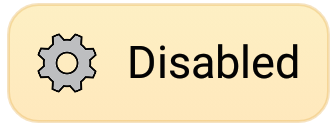
\includegraphics[scale=0.18]{girafbutton_disabled}
        \caption{Disabled}
        \label{fig:girafbutton_disabled}
    \end{subfigure}
    
    \caption{Sates of a button}
    \label{fig:girafbutton_states}
\end{figure}

\todo[inline]{\textbf{OBS!} the disabled button does not at the moment reduce the opacity on the content of the button only the background.}

\section{Content}
\label{sec:button_content}
\index{Button!Content}

A button can either contain text (\figref{fig:girafbutton_text}), and icon (\figref{fig:girafbutton_icon}) or both as seen in (\figref{fig:girafbutton_both}). If one wants a button that does something that can be symbolized easily with an icon (See \charef{cha:sec:icons_and_when_to_use_them}) which the user is familiar with, one should use an icon only button. In other cases where some text is needed to explain an action one should do so, how ever one should only have both icon and text in cases where the icon helps to understand the text. In the cases where there are no icon symbolizing what the text describes one should use a text only button.

\begin{figure}[!htbp]
    \centering

    \begin{subfigure}[t]{0.3\textwidth}
    	\centering
        
\includegraphics[scale=0.18]{girafbutton_text}
        \caption{Button with text}
        \label{fig:girafbutton_text}
    \end{subfigure}
    \hspace{1em} 
    \begin{subfigure}[t]{0.3\textwidth}
    	\centering
        
\includegraphics[scale=0.18]{girafbutton_icon}
        \caption{Button with icon}
        \label{fig:girafbutton_icon}
    \end{subfigure}
    \hspace{1em} 
    \begin{subfigure}[t]{0.3\textwidth}
    	\centering
        
\includegraphics[scale=0.18]{girafbutton_both}
        \caption{Button with both}
        \label{fig:girafbutton_both}
    \end{subfigure}
    
    \caption{Content of a button}
    \label{fig:girafbutton_content}
\end{figure}

\section{Context}
\label{sec:button_context}
\index{Button!Context}

When a collection of buttons is shown regarding the same context the buttons should be ordered by negative and positive actions. Leftmost buttons should cause negative actions and the rightmost should cause positive buttons. An example of this can be seen in the dialog displayed in \figrefpage{fig:profiles_selector_dialog}.

%!TEX root = ../../main.tex
\chapter{Progress Bar}
\label{cha:progress_bar}

The Android framework includes a widget called \androidinline{ProgressBar} which can be used both as an activity indicator (see Figure \ref{fig:dialog_waiting}), and as an actual progress bar. Both usages of the word will henceforth be referred to as just \androidinline{ProgressBar}, unless otherwise made explicit. Both are great at indicating that the application is not frozen and that something is going on. The ProgressBar (as a progress bar) should generally be used when there is a reliable way of calculating the actual progress on the running task. The Activity indicator should generally be used when there is no way of telling how long there will be until the task is complete. \\

%!TEX root = ../../main.tex

\chapter{Dialog}
\label{cha:dialog}


When the user has to respond to a specific event, dialogs should be used. A dialog consistes of a title, a description, some buttons and possibly some additional views. In \gc there exists some classes for this purpose. The general layout of a dialog can be seen in Figure \ref{fig:inflatable_dialog}.

\section{Confirm dialog}
\label{sec:confirm_dialog}

When a user needs to confirm that some action is going to happen, the confirm dialog should be used as it looks in Figure \ref{fig:confirm_dialog}. \todo{refer to appendix}

\begin{figure}[h]
	\centering
	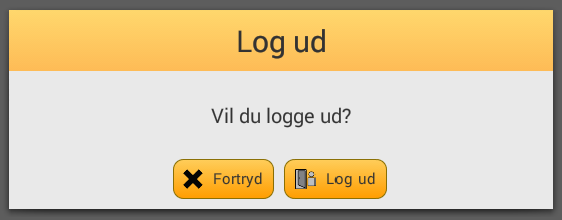
\includegraphics[width=0.4\textwidth]{dialog_confirm}
	\caption{Confirm dialog}
	\label{fig:confirm_dialog}
\end{figure}
\FloatBarrier

\section{Notify dialog}
\label{sec:notify_dialog}

When a user needs to be notified that some action has happened, the notify dialog should be used as it looks in Figure \ref{fig:notify_dialog}. \todo{refer to appendix}

\begin{figure}[h]
	\centering
	
\includegraphics[width=0.4\textwidth]{dialog_notify}
	\caption{Notify dialog}
	\label{fig:notify_dialog}
\end{figure}
\FloatBarrier

\section{Profileselector Dialog}
\label{sec:profileselector_dialog}

When a user needs to select a profile in some context, eg. change the current citizen on the tablet one should use the dialog as it looks in Figure \ref{fig:profile_selector_dialog}. In other usecases a user might need to select multiple profiles, one should use the profile as it looks in Figure \ref{fig:profiles_selector_dialog}. \todo{refer to appendix}.

\begin{figure}[!htbp]
    \centering
    \begin{subfigure}[t]{0.4\textwidth}
    	\centering
        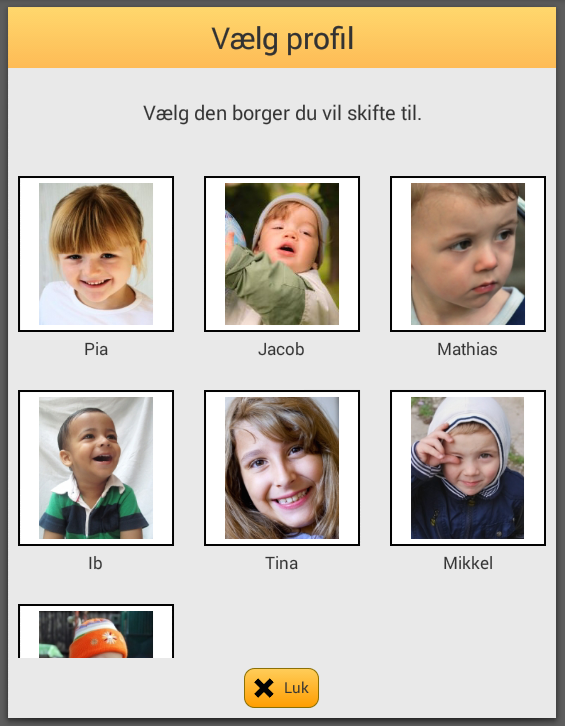
\includegraphics[scale=0.3]{dialog_profile_selector}
        \caption{Single profile selector}
        \label{fig:profile_selector_dialog}
    \end{subfigure}
    \hspace{5em}
    \begin{subfigure}[t]{0.4\textwidth}
    	\centering
        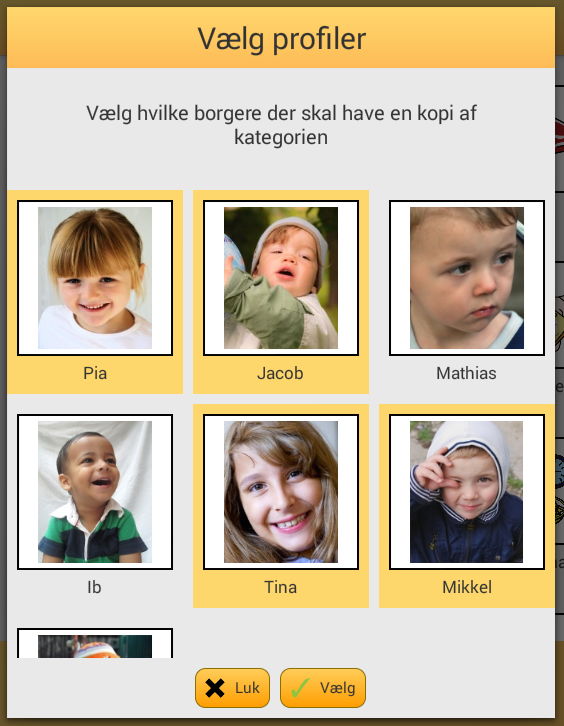
\includegraphics[scale=0.3]{dialog_profiles_selector}
        \caption{Multi profile selector}
        \label{fig:profiles_selector_dialog}
    \end{subfigure}
    
    \caption{Profile selectors}
    \label{fig:profile_selection}
\end{figure}

\section{Waiting Dialog}
\label{sec:waiting_dialog}

In cases where the system needs to peform some action that takes a long task (Section \ref{sub:long_tasks}, to indicate that the system is not frozen the waiting dialog, as it looks in Figure \ref{fig:dialog_waiting}, can be used. \todo{refer to appendix}.

\begin{note}
	If one have temporally unused screen real estate at the location where one are conceptually loading in elements then you should place you progress bar or activity indicator in this unused screen real estate. A waiting dialog should only be used in the case when there are not enough screen estate awailable or in cases where it does not make sense to display a progressbar in the unused screen estate. An activiy indiactor as the progressbar should generally be used when there is no way of telling how long there will be til the task is complete. 
\end{note}


\begin{figure}[h]
	\centering
	
\includegraphics[width=0.4\textwidth]{dialog_waiting}
	\caption{Waiting dialog}
	\label{fig:dialog_waiting}
\end{figure}
\FloatBarrier

\subsection{Long Tasks}
\label{sub:long_tasks}
Long running tasks should generally not block the GUI. Any task that can potentially take a long time should be done on a background thread and NOT on the main GUI thread see Appendix \ref{app:threading_asynctask}. 

\section{Inflatable Dialog}
\label{sec:inflatable_dialog}

Some uses of dialogs might be more specific than the ones already existing in \gc, for this reason the inflatable dialog exists. If one wants to add input fields or a custom view one should use this dialog. In Figure \ref{fig:inflatable_dialog}, an example of dialog is shown, this example shows the usecase when a user needs to edit a category.

\begin{figure}[h]
	\centering
	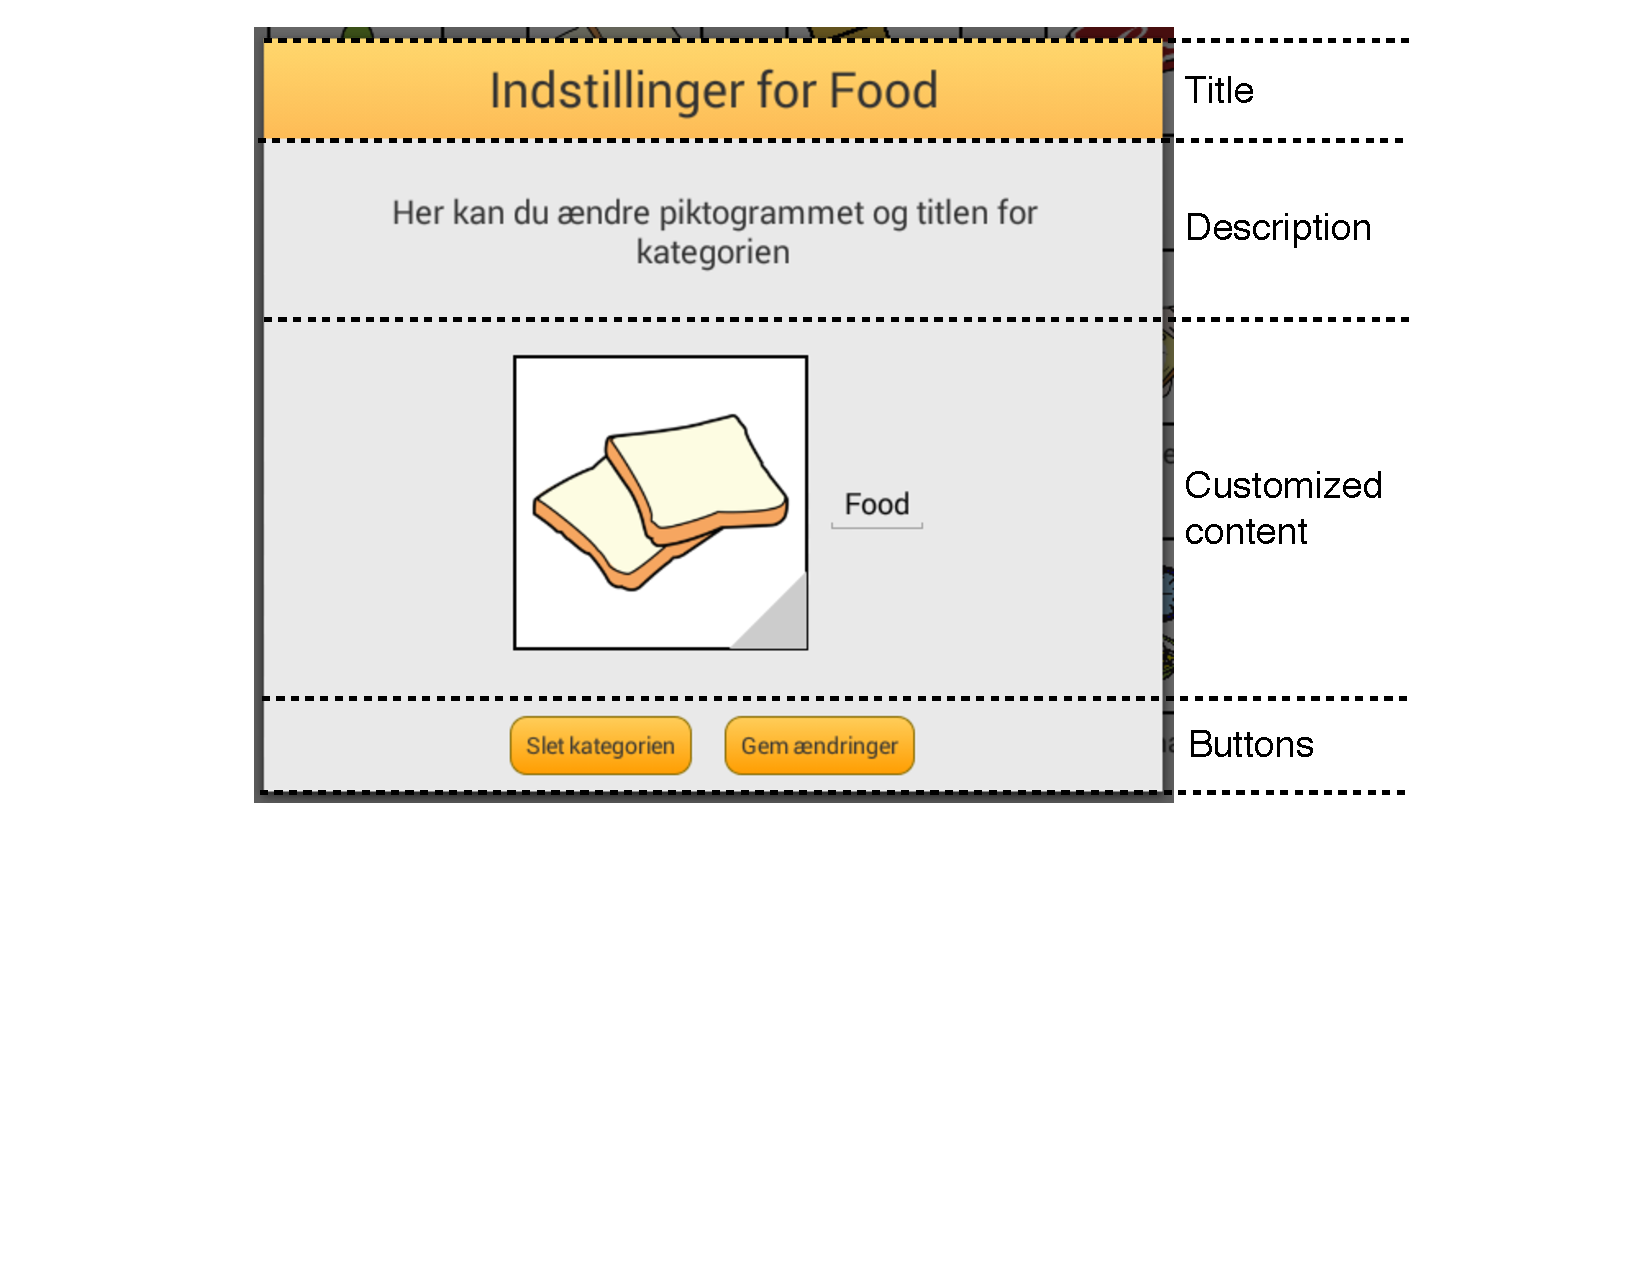
\includegraphics[width=0.6\textwidth]{dialog_inflatable}
	\caption{Inflatable dialog}
	\label{fig:inflatable_dialog}
\end{figure}
\FloatBarrier

\begin{note}
	It is important that if buttons should be added to this type of dialog it must be placed in the very bottom of the dialog and should be divided as shown in Figure \ref{fig:inflatable_dialog}.
\end{note}







%!TEX root = ../../main.tex

\chapter{Tabs}
\label{cha:tabs}

\todo[inline]{\textbf{Describe Tabs:} The design of tabs should be consistent around the giraf software suite. How ever at the moment they only exist in the launcher. There exist both horizontal tabs and vertical tabs in the launcher. Other apps could use these tabs to improve the usability.}

%!TEX root = ../../main.tex

\chapter{Spinners}
\label{cha:spinners}

\todo[inline]{\textbf{Describe Spinners (GirafSpinner):} This is also known as a dropdown menu. Describe how this should look like, and describe how to inser text into it. Create an appendix that describes how one uses GirafSpinner and GirafSpinnerAdapter. The spinner is not well implemented, but some soloution already exist called a GirafSpinner}

\begin{figure}[h]
	\centering
	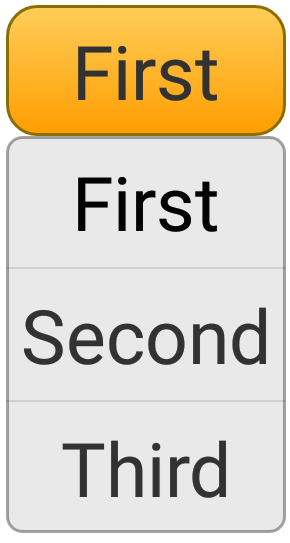
\includegraphics[width=0.1\textwidth]{girafspinner}
	\caption{Current implementation \androidinline{GirafSpinner}}
	\label{fig:girafspinner}
\end{figure}

%!TEX root = ../../main.tex

\chapter{Sequences}
\label{cha:sequences}

A sequence is a list of pictograms, where it is possible to mark a progress in the sequence of pictograms. This components is very common in the Sekvens app and the Ugeplan app.

\section{Progress}
\label{sec:progress}

The progress of the sequence is indicated by the size of pictograms in the sequence. The pictogram currently in progress is always in the middle of the view displaying the sequence as seen in \figref{fig:sequence_progress}. When displaying pictograms to a citizen it may not split (\secref{sub:citizen_view}). Upcomming pictograms should be a bit smaller than the one currently in progress. When progress has been made the pictograms that are done should be smaller and grayed as seen in \figref{fig:sequence_two} and \figref{fig:sequence_three}. For the ratio between the pictograms see \tabref{tab:sequence_ratio}.

\begin{figure}[!htbp]
    \centering

    \begin{subfigure}[t]{0.27\textwidth}
    	\centering
        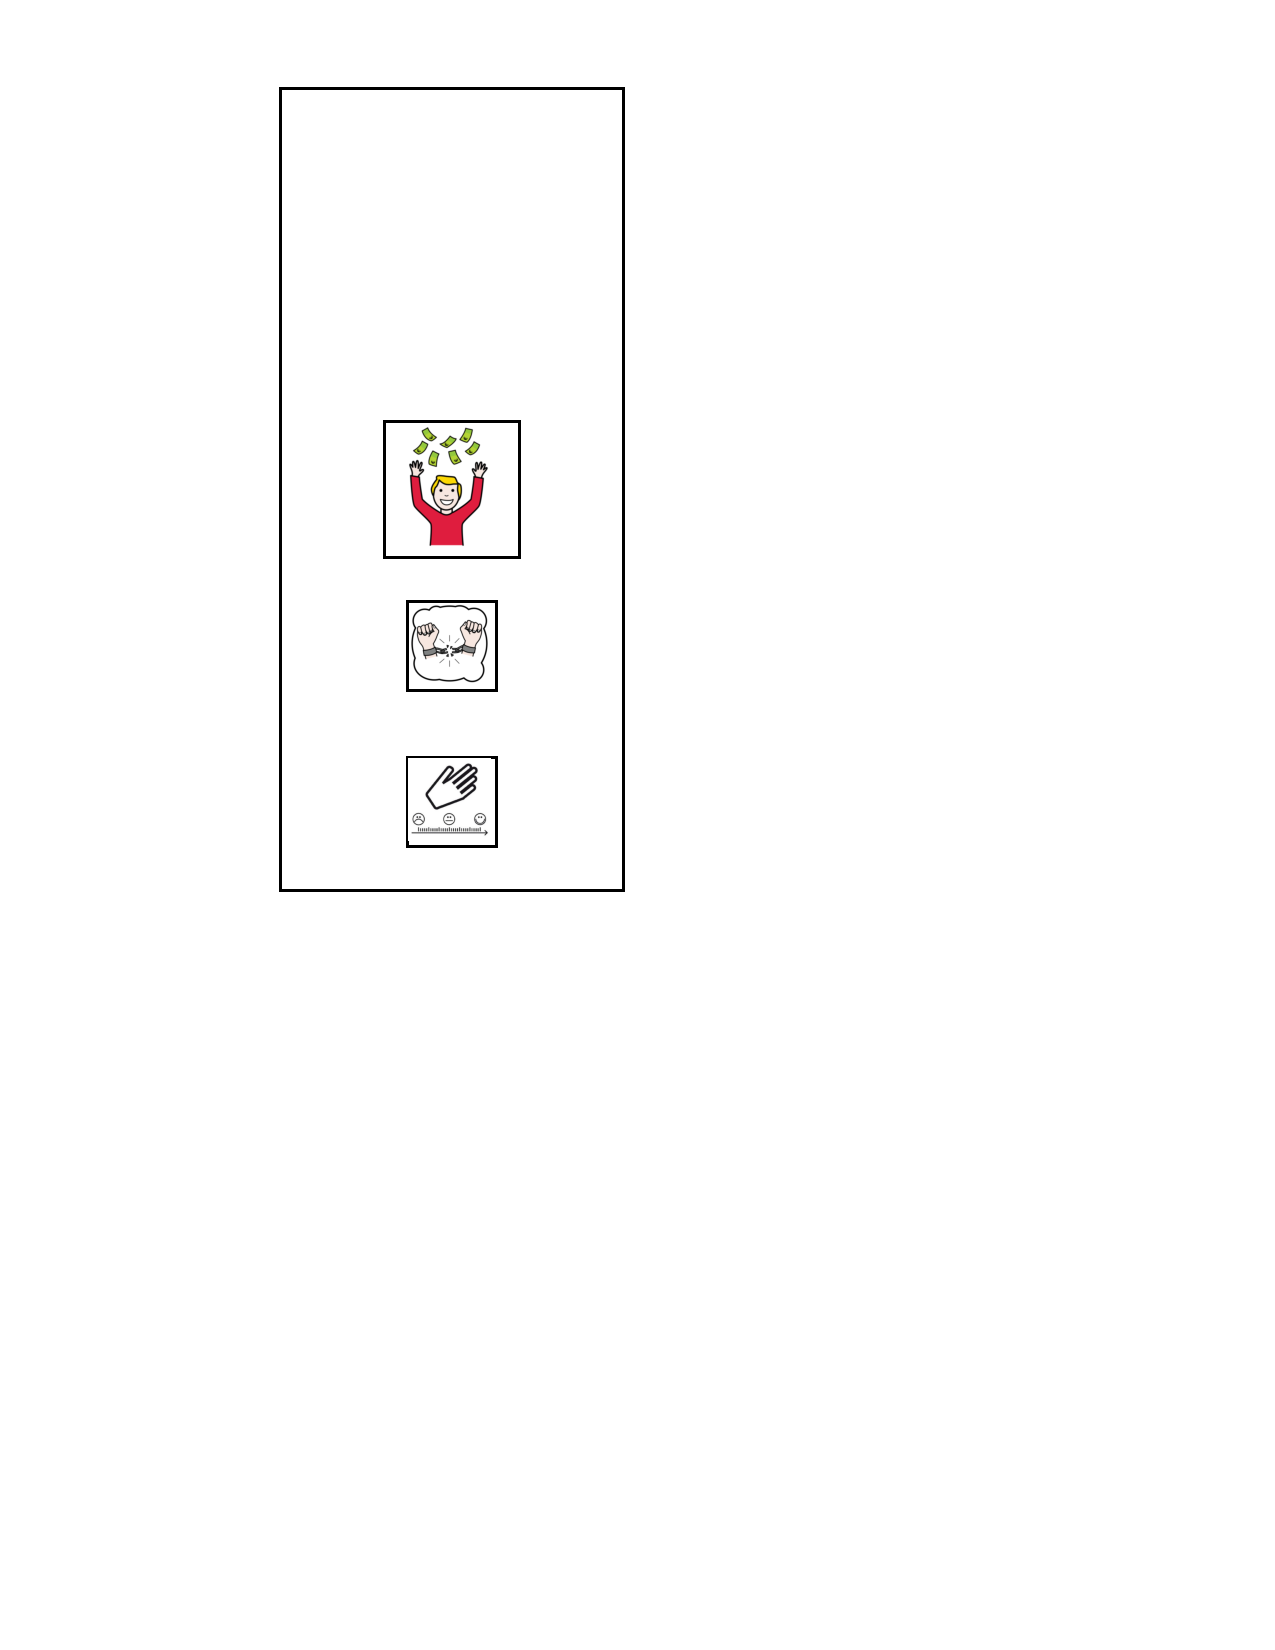
\includegraphics[scale=0.3]{sequence_one}
        \caption{Start of sequence}
        \label{fig:sequence_one}
    \end{subfigure}
    \hspace{2em} 
    \begin{subfigure}[t]{0.27\textwidth}
    	\centering
        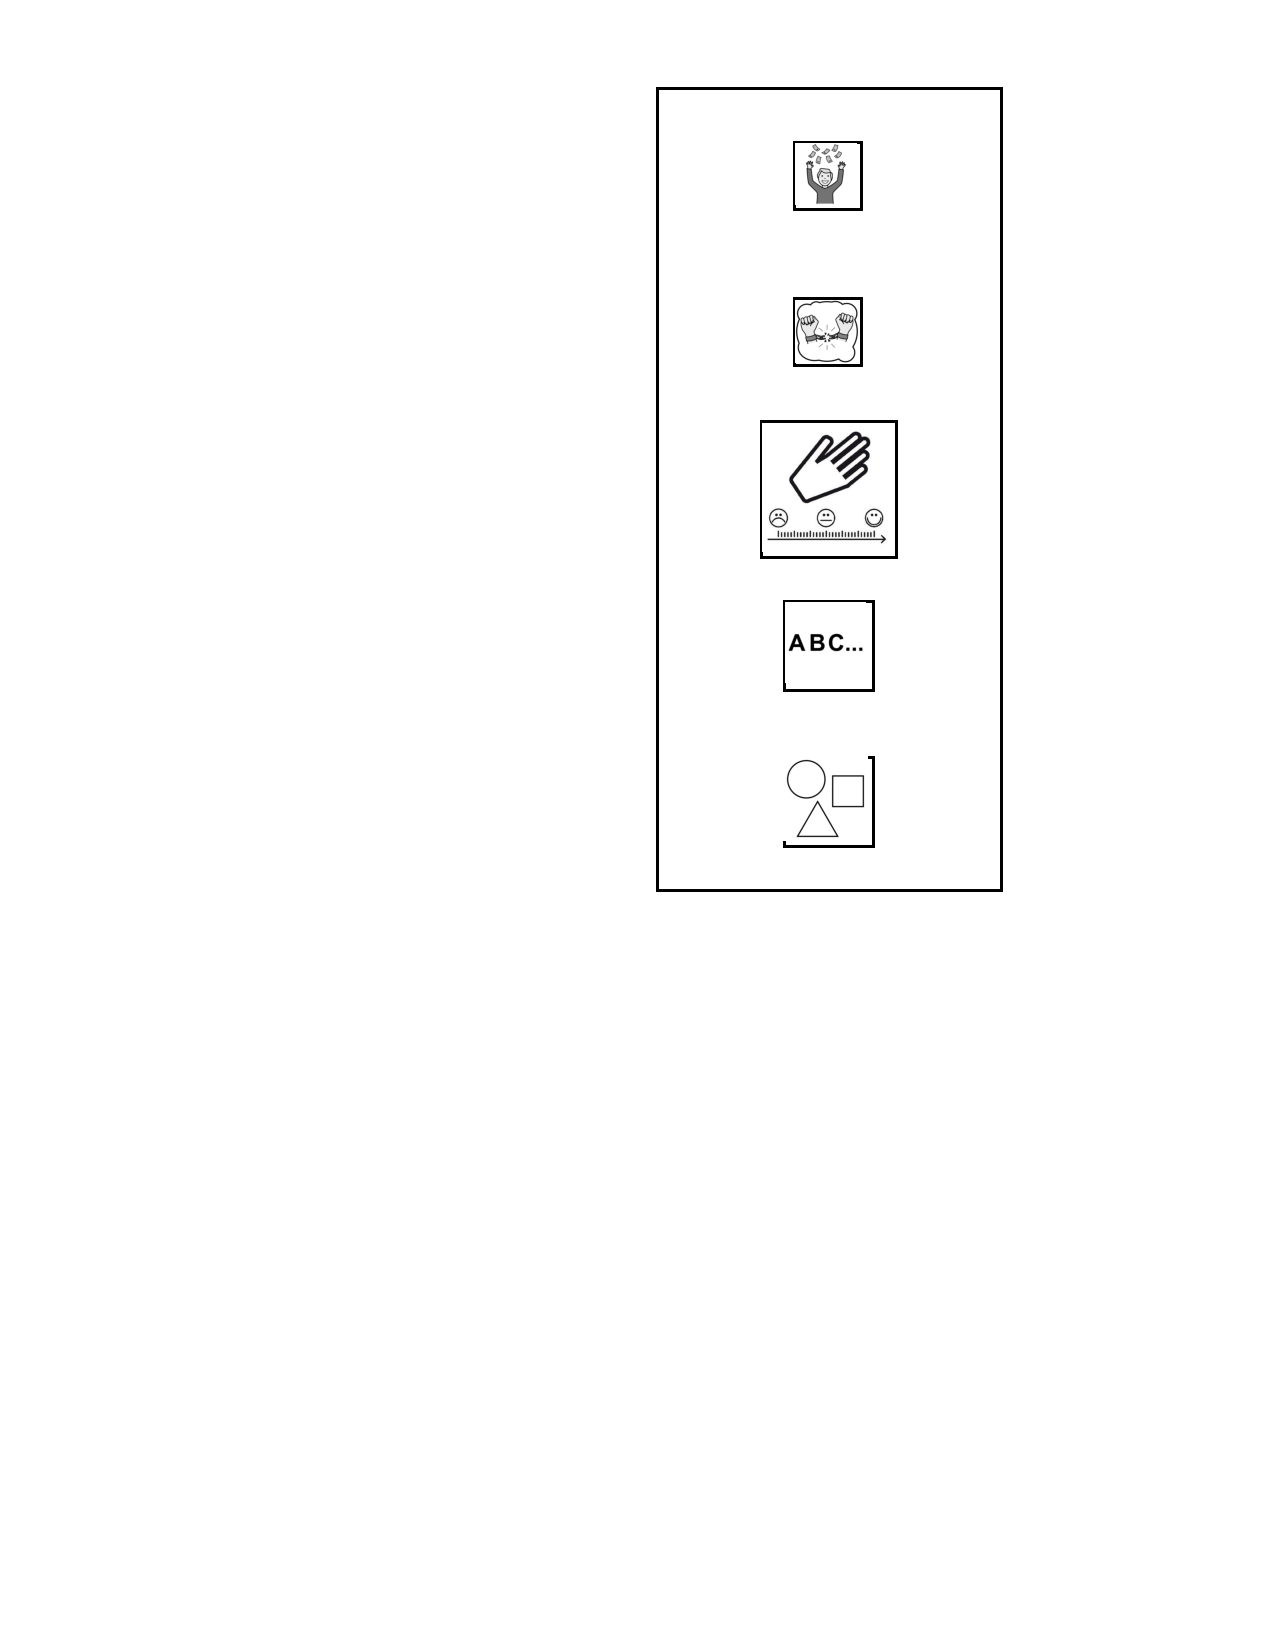
\includegraphics[scale=0.3]{sequence_two}
        \caption{Middle of sequence}
        \label{fig:sequence_two}
    \end{subfigure}
    \hspace{2em} 
    \begin{subfigure}[t]{0.27\textwidth}
    	\centering
        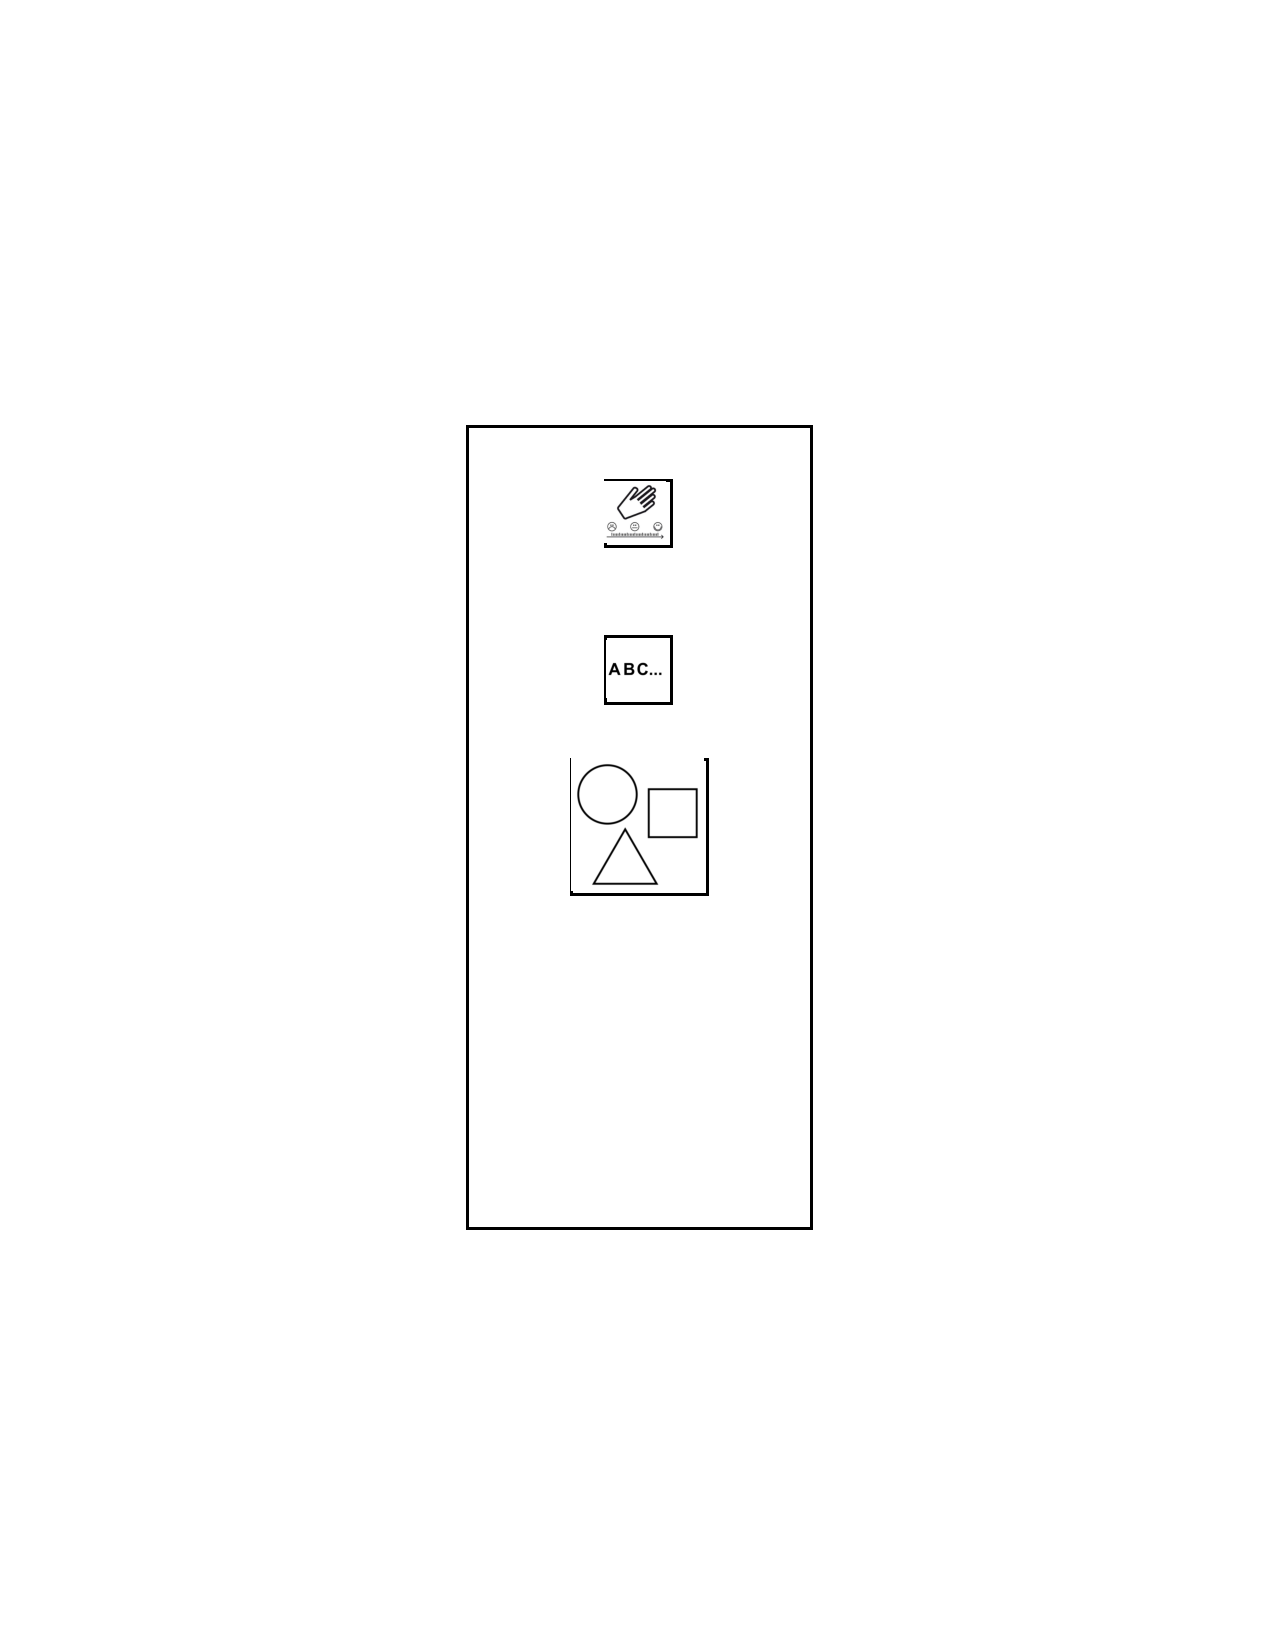
\includegraphics[scale=0.3]{sequence_three}
        \caption{End of sequence}
        \label{fig:sequence_three}
    \end{subfigure}
    
    \caption{Sequence progress}
    \label{fig:sequence_progress}
\end{figure}

\begin{table}[!htbp]
	\centering
	\begin{tabular}{|l|c|c|c|}
		\hline
		~ & Upcomming & In Progress & Done \\ \hline
		Ratio & 1 & 1.5 & 0.75 \\ \hline
	\end{tabular}
	\caption{Sequence picotgrams ratio}
    \label{tab:sequence_ratio}
\end{table}



%----------------------------------------------------------------------------------------
%	APPENDIX
%----------------------------------------------------------------------------------------
\part{Appendix}
\appendix
%!TEX root = ../../main.tex

%!TEX root = ../../../main.tex
\chapter{Customization of action bar}
\label{app:customization_of_action_bar}

If one wants to customize the action bar, the \androidinline{GirafActivity} provides the possibility to change the title of the action bar and the possibility of adding \androidinline{GirafButton}s to the action bar. The action bar looks like the one in \figrefpage{fig:top_bar_example}. 

\begin{note}
    This actionbar is only available to activities that extends the \androidinline{GirafActivity}.
\end{note}

\noindent
From default the title in the top bar is the label of the application, how ever if one wants to customize it the \androidinline{setActionBarTitle} method can be used as seen in \lstrefline{lst:customized_action_bar}{line:actionbar:title}.
\\\\
The action bar always have a back button shown that does the same as the standard android back button. If one wants to add more buttons to the action bar one can use the \androidinline{addGirafButtonToActionBar} method. One can then instantiate some \androidinline{GirafButton}s and then use this method as in \lstreflines{lst:customized_action_bar}{line:actionbar:buttonstart}{line:actionbar:buttonend}

\lstinputlisting[
    style = java,
    caption = {Customized action bar},
    label = {lst:customized_action_bar},
]{content/appendix/customization_of_action_bar/ExampleActivity.java}


%!TEX root = ../../../main.tex
\chapter{Usage of GirafButtons}
\label{cha:usage_of_girafbuttons}

\todo[inline]{Update to the new giraf button}

\lstinputlisting[
    style = java,
    caption = {Customized action bar},
    label = {lst:customized_action_bar},
]{content/appendix/usage_of_girafbuttons/ExampleActivity.java}

\lstinputlisting[
    style = java,
    caption = {Customized action bar},
    label = {lst:customized_action_bar},
]{content/appendix/usage_of_girafbuttons/example_activity.xml}

%!TEX root = ../../../main.tex
\chapter{Implementation Guide for Dialogs}
\label{cha:implementation_guide_for_dialogs}

When using the various dialogs implemented in the \gc, it is important that one uses the support library, this is done by including the support library in the gradle build file as seen in \lstref{lst:build_gradle}.

\lstinputlisting[
    style = gradle,
    caption = {build.gradle},
    label = {lst:build_gradle},
]{content/appendix/implementation_guide_for_dialogs/code_snippets/build.gradle}
\noindent
The dialogs is an extension of the android class \androidinline{DialogFragment}, meaning that all dialogs is handled as fragments. This means that callbacks from the dialogs is done using interfaces, which the activity starting them should implement. Through out the description of these dialogs there will be talked about a method called \androidinline{onActionButtonClick} which is an event that is called whenever some gui element is clicked, eg. when a button is clicked. This method will in all of the following examples create an instance of the dialog and show it using the \androidinline{show} method.
\\\\
Also note that in all of the following code snippets there is declared a string tag (\androidinline{DIALOG_TAG}) this is a tag that the Android system needs to handle fragments. However in many of the code snippets there also exist an integer (\androidinline{DIALOG_ID}) which is used to call a method in the activity from the fragment.

\begin{note}
	It is important that whenever one creates a dialog one uses the \androidinline{newInstance} method on the specific dialog.
\end{note}

\begin{note}
    Remember to call the \androidinline{show} method on the dialog when the dialog should be displayed. Simply instantiating it is not enough.
\end{note}

\begin{note}
    It is important to check that it is the correct \androidinline{dialogIdentifier} that is used in the methods implemented from interfaces in order to determine which dialog was actually responded to. 
\end{note}

\section{Confirm dialog}
\label{sec:impl_confirm_dialog}

The confirm dialog is used to make the user confirm an action before it is executed. This section describes how one could implement an confirm dialog as described in \secref{sec:confirm_dialog}. An example of such an implementation can be seen in \lstref{lst:impl_confirm_dialog}.
\\\\
Using the \androidinline{GirafConfrimDialog.Confirmation} interface (\lstrefline{lst:impl_confirm_dialog}{line:confirm_dialog:interface}) allows the activity (\androidinline{ExampleActivity}) to implement the method \androidinline{confirmDialog}, as in \lstrefline{lst:impl_confirm_dialog}{line:confirm_dialog:confirmdialogstart}, that will be called from the dialog whenever a response has been made for it (when the user press the acceptance button).  

\lstinputlisting[
    style = java,
    caption = {Implementaion of confirm dialog},
    label = {lst:impl_confirm_dialog},
]{content/appendix/implementation_guide_for_dialogs/code_snippets/confirm_dialog.java}

\noindent
The default behavior of buttons in the dialog is to dismiss it. The acceptance button will furthermore call the \androidinline{confirmDialog} with the identifier \androidinline{CONFIRM_DIALOG_ID}, as in \lstreflines{lst:impl_confirm_dialog}{line:confirm_dialog:confirmdialogstart}{line:confirm_dialog:confirmdialogend}.

\section{Notify dialog}
\label{sec:impl_notify_dialog}
The notify dialog is used to make the user aware of some event. This section described how one could implement an notify dialog as described in \secref{sec:notify_dialog}. An example of such an implementation can be seen in \lstref{lst:impl_notify_dialog}.
\\\\
Using the \androidinline{GirafNotify.Notification} interface (\lstrefline{lst:impl_confirm_dialog}{line:notify_dialog:interface}) allows the activity (\androidinline{ExampleActivity}) to implement the method \androidinline{noticeDialog}, as in \lstrefline{lst:impl_notify_dialog}{line:notify_dialog:noticedialogstart}, that will be called from the dialog whenever a response has been made for it (when the user press the button).  

\lstinputlisting[
    style = java,
    caption = {Implementaion of notify dialog},
    label = {lst:impl_notify_dialog},
]{content/appendix/implementation_guide_for_dialogs/code_snippets/notify_dialog.java}

\noindent
The default behavior the button in the dialog is to dismiss it. The button will furthermore call the \androidinline{confirmDialog} with the identifier \androidinline{NOTIFY_DIALOG_ID}, as in \lstreflines{lst:impl_confirm_dialog}{line:notify_dialog:noticedialogstart}{line:notify_dialog:noticedialogend}.

\section{Profileselector dialog}
\label{sec:impl_profileselector_dialog}

The profile selector dialog is used to allow for user to select one ore more profiles. This section describes how one could implement an confirm dialog as described in \secref{sec:profileselector_dialog}. Examples of such an implementation can be seen in \lstref{lst:impl_single_profileselector_dialog} and \lstref{lst:impl_multi_profileselector_dialog}.
\\\\
This dialog is used in two use cases. One where the user wants to select exactly one profiles, and another use case where one wants to select arbitrary many profiles. Using the \androidinline{GirafProfileSelectorDialog.OnSingleProfileSelectedListener} interface allows for the activity (\androidinline{ExampleActivity}) to respond on a single selected profile as in \lstrefline{lst:impl_single_profileselector_dialog}{line:single_profile_selector:interface}. Where as the \androidinline{GirafProfileSelectorDialog.OnMultipleProfilesSelectedListener} allows for the activity to respond on multi selected profiles an in \lstrefline{lst:impl_multi_profileselector_dialog}{line:multi_profile_selector:interface}.
\begin{note}
    Observe that the main difference between the instantiating of the single and multi version of the profile selector dialog is the fourth argument called \androidinline{selectMultipleProfiles}. That determines which interface will be called. If this boolean is set to \androidinline{true} the activity should implement \androidinline{GirafProfileSelectorDialog.OnMultiProfileSelectedListener} otherwise the activity should implement \androidinline{GirafProfileSelectorDialog.OnSingleProfileSelectedListener}. Obviously if an activity have one dialog of each type both interfaces should be implemented.
\end{note}

\lstinputlisting[
    style = java,
    caption = {Implementaion of single profile selector dialog},
    label = {lst:impl_single_profileselector_dialog},
]{content/appendix/implementation_guide_for_dialogs/code_snippets/single_profile_selector_dialog.java}

\noindent
When a profile is clicked in a single profile selector the \androidinline{onProfileSelected} method is called, with the profile that was selected and the identifier \androidinline{PROFILE_SELECT_DIALOG_ID} as in \lstreflines{lst:impl_single_profileselector_dialog}{line:single_profile_selector:onprofileselectedstart}{line:single_profile_selector:onprofileselectedend}.

\lstinputlisting[
    style = java,
    caption = {Implementaion of multi profile selector dialog},
    label = {lst:impl_multi_profileselector_dialog},
]{content/appendix/implementation_guide_for_dialogs/code_snippets/multi_profile_selector_dialog.java}

\noindent
When a profile is clicked in a multi profile selector the \androidinline{onProfilesSelected} method is called, with a list of profiles and a boolean telling of they were marked or not alongside the identifier \androidinline{PROFILE_SELECT_DIALOG_ID} as in \lstreflines{lst:impl_multi_profileselector_dialog}{line:multi_profile_selector:onprofilesselectedstart}{line:multi_profile_selector:onprofilesselectedend}.

\section{Waiting dialog}
\label{sec:impl_waiting_dialog}

The waiting dialog is used to indicate to the user that some task is being executed and that he/she should wait for that task to end. This section describes how one could implement an waiting dialog as described in \secref{sec:waiting_dialog}.

\begin{note}
    Note that in this dialog the dialog is instantiated in the \androidinline{onCreate} method (see \lstrefline{lst:impl_waiting_dialog}{line:waiting_dialog:oncreate}), and is called showed implicitly by the \androidinline{onActionButtonClick} method which starts the async task (see \lstrefline{lst:impl_waiting_dialog}{line:waiting_dialog:executetask}.
\end{note}

\noindent
This dialog is often used when some thread syncing tasks is running (see \appref{app:threading_asynctask}). This dialog requires not interface to work properly. Good practice with this dialog is to show it before the long task is executed. This can be done using the \androidinline{onPreExecute} method (see \lstrefline{lst:impl_waiting_dialog}{line:waiting_dialog:showdialog}). One should dismiss the dialog after the task is done which can be handled in \androidinline{onPostExecute} method (see \lstrefline{lst:impl_waiting_dialog}{line:waiting_dialog:dismissdialog}).

\lstinputlisting[
    style = java,
    caption = {Implementaion of waiting dialog},
    label = {lst:impl_waiting_dialog},
]{content/appendix/implementation_guide_for_dialogs/code_snippets/waiting_dialog.java}

\section{Custom buttons dialog}
\label{sec:impl_custom_buttons}

The custom buttons dialog is used when the developer wants to provide the user with more than two buttons in the dialog. This section described how one coul dimplement an custom buttons dialog as described in \secref{sec:custom_buttons_dialog}.
\\\\
Using the \androidinline{GirafCustomButtonsDialog.CustomButtons} (\lstrefline{lst:impl_custom_buttons}{line:custom_buttons_dialog:interface}) interface allows for the developer to add abitrary many buttons to the dialog.

\begin{note}
    There is no limit on buttons that can be added to the dialog, but one should be careful that the design is consistent. The width should not exceed the width of other dialogs.
\end{note}

\lstinputlisting[
    style = java,
    caption = {Implementaion of custom buttons dialog},
    label = {lst:impl_custom_buttons},
]{content/appendix/implementation_guide_for_dialogs/code_snippets/custom_buttons_dialog.java}

\noindent
Before the dialog is created the \androidinline{fillButtonContainer} method is called, see \lstreflines{lst:impl_custom_buttons}{line:custom_buttons_dialog:fillbuttonstart}{line:custom_buttons_dialog:fillbuttonend}. The identifier \androidinline{CUSTOM_BUTTONS_DIALOG_ID} determines which dialog is being filled with buttons.

\section{Inflatable dialog}
\label{sec:impl_inflatable_dialog}

The inflatable dialog is used to create more custom dialogs and want some custom gui elements to be shown in the dialog. In this example we have created a custom dialog that contains an AnalogClock element and a button to dismiss the dialog.
\\\\
When creating an instance of this type of dialog the \androidinline{newInstance} method takes an layout resource as third argument. The argument \androidinline{R.layout.example} as seen in \lstrefline{lst:impl_inflatable_dialog}{line:inflatable_dialog:layoutres} comes from the layout seen in \lstref{lst:impl_inflatable_dialog_layout}.

\lstinputlisting[
    style = java,
    caption = {The implementation of the inflatable dialog},
    label = {lst:impl_inflatable_dialog},
]{content/appendix/implementation_guide_for_dialogs/code_snippets/inflatable_dialog.java}

\noindent
Using the \androidinline{GirafInflatableDialog.OnCustomViewCreatedListener} interface (\lstrefline{lst:impl_inflatable_dialog}{line:inflatable_dialog:interface}) allows for the developer to access the custom created layout by the \androidinline{editCustomView} method. See \lstreflines{lst:impl_inflatable_dialog}{line:inflatable_dialog:accesscustomviewstart}{line:inflatable_dialog:accesscustomviewend} for an example of how one access the custom view. 

\begin{note}
    One cannot access the custom inflated view before the \androidinline{editCustomView} is called from the dialog it self.
\end{note}

\lstinputlisting[
    style = xml,
    caption = {The custom layout for an inflateable dialog},
    label = {lst:impl_inflatable_dialog_layout},
]{content/appendix/implementation_guide_for_dialogs/code_snippets/example_layout.xml}


%!TEX root = ../../../main.tex

\chapter{Implementation Guide for Pictures}
\label{cha:implementation_guide_for_pictures}

To accommodate the need for displaying pictures throughout the different applications in the \giraf software suite, a shared component was build in the \gc library. This chapter will cover the use and functionality of this component. The component implemented is named \androidinline{GirafPictogramItemView}.

\todo[inline]{Consider if it would be better to rename it to something like \androidinline{GirafImageEntityView} to indicate that the component may be used to more than just displaying pictograms}

\begin{note}
    Throughout this chapter different examples will reference constructors of the \androidinline{GirafImageEntityView}. The class contains a lot of different constructors with a lot of different, optional, parameters. The examples will only cover some of these constructors, so please reference the documentation for the class if in doubt.
\end{note}

\section{General Usage}
\label{sec:general_usage}
The component may be used to display anything that extends the \androidinline{ImageEntity}-interface. Examples of such classes are \androidinline{Pictogram}, \androidinline{Category}, and \androidinline{Applications}. This section will only cover the most basic use of the component. Please refer to the following sections to see more specific usages of the components.

\todo[inline]{Write that the only use for this component is programmatically and it's XML implementations are very limited}

\begin{note}
    Some classes cannot be used because of a poor structure. Example of such a class is \androidinline{Sequence}, which does not have its own image but instead a reference to a \androidinline{Pictogram}. When using the the component, please make sure that the class extends the \androidinline{ImageEntity} interface otherwise refer to \secref{sec:workarounds} to see how to fix this issue.
\end{note}

\noindent
The most general use of this component is to simply display an image. This image ``comes from'' objects (instances) of classes that extend the \androidinline{ImageEntity}. To create a new instance of the view, simply call its constructor which will require a context and the object that should be displayed. \lstref{lst:basic_use} shows an example of a \androidinline{getView}-method in an adapter which is used to display pictograms. Please note that this example does not include a title below the picture. To do this, additional parameters for the constructors are required. \lstref{lst:basic_use_with_title} shows the same example, however including the title parameter. The title can also later be changed (or set) using the \androidinline{setTitle}-method on the \androidinline{GirafPictogramItemView} object. The title can furthermore be shown or hidden using the methods \androidinline{showTitle} and \androidinline{hideTitle}.
 
\lstinputlisting[
    style = java,
    caption = {Basic use},
    label = {lst:basic_use},
]{content/appendix/implementation_guide_for_pictures/code_snippets/basic_use.java} 

\lstinputlisting[
    style = java,
    caption = {Basic use (with title)},
    label = {lst:basic_use_with_title},
]{content/appendix/implementation_guide_for_pictures/code_snippets/basic_use_with_title.java} 


\section{Indicator Overlay}
\label{sec:indicator_overlay}
In some situations it may be required to indicate something about a picture - for instance when differentiating between pictograms and categories or that the picture can be edited. This can be achieved by using a small indicator overlay in the bottom right corner of the picture. (See \secref{sec:indicator_overlay} for additional information). 

\subsection{Overlay to indicate editable status}
To indicate that a picture is editable use the method \androidinline{setEditable} on a \androidinline{GirafPictogramItemView} object. This method requires a \androidinline{boolean} as argument. If set to \androidinline{true}, the picture will appear as editable, while \androidinline{false} will display the picture as normal.

\subsection{Custom indicator overlay}
To use a custom indicator overlay, use the method \androidinline{setIndicatorOverlayDrawable} on a \androidinline{GirafPictogramItemView} object. This method requires a \androidinline{Drawable} as argument. 

\begin{note}
    It is not possible to use both an editable-overlay along with a custom indicator. If you try to do this, you will receive an exception.
\end{note}


\section{Fallback Drawable}
\label{sec:fallback_drawable}
If you suspect that some of the \androidinline{ImageEntity}-objects does not actually have an image, a fallback-image may be used. This fallback image will only be displayed in the case that the original objects does not have any images. \lstref{lst:usage_with_fallback} shows an example of a \androidinline{getView}-method in an adapter. This example will use the drawable \androidinline{icon_fallback} if the variable \androidinline{pictogram} does not have an image. 
\\\\
The fallback drawable can also be set when calling the \androidinline{setImageModel}-method. This method require two parameters, the first being an \androidinline{ImageEntity} (the object that should be shown) and the second is a \androidinline{Drawable}, which will be used as a fallback.

\lstinputlisting[
    style = java,
    caption = {Usage with fallback},
    label = {lst:usage_with_fallback},
]{content/appendix/implementation_guide_for_pictures/code_snippets/fallback.java} 


\section{Grayscaled Pictures}
\label{sec:grayscaled_pictures}
If needed, the \androidinline{GirafPictogramItemView} can display all of the pictures grayscaled. From default, this is disabled but may be enabled by adding an additional boolean parameter (set to true) to the constructor or by adding the same parameter to the \androidinline{setImageModel}-method.


\section{Marking}
\label{sec:marking}
Marking of \androidinline{GirafPictogramItemView} can be done through one of the following methods. The method \androidinline{setChecked} requires a boolean, indicating if the view should be marked (\androidinline{true}) or not (\androidinline{false}). \androidinline{toggle} required no parameters and will simply invert the current checked/marked state. If needed, you may call \androidinline{isChecked} which will return a \androidinline{boolean} indicating if the view is marked. 


\section{Workarounds}
\label{sec:workarounds}

\begin{note}
    These workarounds are not something that should be used ideally, and should only be temporarily fixes until the structure of the different classes are fixed. This workaround only works for classes that do not implement the interface \androidinline{ImageEntity}. If the class that you want to display implements \androidinline{ImageEntity}, please refer to \secref{sec:general_usage}.    
\end{note}

\noindent
Most classes that do not implement the interface \androidinline{ImageEntity} have some kind of relation to something that does. So to display the wrongly structured class, you must first locate this relation. For instance when displaying a \androidinline{Sequence}, you must use its reference to a \androidinline{Pictogram} in order to display it. Please refer to \lstref{lst:workaround_example} to see an example of how to implement this workaround.

\lstinputlisting[
    style = java,
    caption = {Workaround example},
    label = {lst:workaround_example},
]{content/appendix/implementation_guide_for_pictures/code_snippets/workaround_example.java} 

%!TEX root = ../../../main.tex
\chapter{Threading AsyncTask}\label{app:threading_asynctask}

This chapter introduces good practice to managing the GUI thread of Android applications.  

\section{Android GUI Thread}
\label{sec:gui_thread_async_task}

The Android system imposes real time constraints on applications to keep them smooth and lag free. This section covers how one should make sure not to violate these constraints across all application code.

\subsection{GUI Thread}
The real time constraints are implemented on a special GUI thread which runs the user interface event loop, which is basically a queue of tasks (Java Runnable). Applications, e.g. activities, in the Android eco system run, i.e updates their views, on this GUI thread. Any updates to views not coming from the GUI thread will result in an exception. In Android, these real time constraints on the GUI thread have been implemented by simply setting a hard limit on how long, in real time, tasks on the GUI thread are allowed to run. Any violation of the constraints will result in an Application Not Responding (ANR) message to the user \footnote{Keeping Your App Responsive - http://developer.android.com/training/articles/perf-anr.html}. Users will not be able to distinguish an unresponsive application, e.g. the result of a deadlock, from a task taking too long on the GUI thread, which may cause the user to terminate an otherwise functioning application that was doing some complicated database query or downloading some file from the Internet. 

\subsection{AsyncTask}

The Android framework provides a very useful abstraction which makes it easy to run long tasks in the background with a class called AsyncTask. The AsyncTask provides four non final methods that make it easy to synchronize between a background thread and the GUI thread. The three methods \androidinline{onPreExecute}, \androidinline{onProgressUpdate}, \androidinline{onPostExecute} are always all guaranteed to run on the GUI thread. The last method, \androidinline{doInBackground}, always runs on an unspecified background thread from a pool of threads maintained by the system. The class then ensures an order on these method calls being: \androidinline{onPreExecute}, \androidinline{doInBackground}, \androidinline{onPostExecute}. The \androidinline{onProgressUpdate} method can be run multiple times while the doInBackground method is running and is started by a call to a method called \androidinline{publishProgress} from the \androidinline{doInBackground} method.  

\subsection{Long Tasks}

Not causing the application to show an ANR message is one thing, making the user explicitly aware that a long task is running, through some kind of feedback, is considered good practice as well \footnote{David Benyon - Designing Interactive Systems 2nd Edition}. We have tried to provide this feedback through Android \androidinline{ProgressBar} widgets whenever long operations take place. The name ``ProgressBar'' is a bit misleading since the style of the \androidinline{ProgressBar} we use, which is the default style, is more like a spinning activity indicator as seen in Figure \ref{fig:dialog_waiting} on Page \pageref{fig:dialog_waiting}. 

%----------------------------------------------------------------------------------------
%	INDEX
%----------------------------------------------------------------------------------------

\part{Index}
\cleardoublepage
\phantomsection
\setlength{\columnsep}{0.75cm}
\addcontentsline{toc}{chapter}{\textcolor{ocre}{Index}}
\printindex

%----------------------------------------------------------------------------------------



\end{document}